% 45 bài Tuyển sinh 10 chuẩn hóa nạp vào ngân hàng lớp 9

\begin{bt}%[9D6H18-2]%[ma:654bf2ee]
% nguon: Tuyển tập đề thi Tuyển sinh 10 TP.HCM
Cho parabol $(P): y = \frac{1}{2}x^2$.
\textbf{a)} Vẽ đồ thị $(P)$ trên hệ trục tọa độ. \par
\textbf{b)} Tìm tọa độ các điểm $M$ thuộc $(P)$ (khác gốc tọa độ $O$) sao cho tung độ của điểm $M$ gấp đôi hoành độ của nó.
\loigiai{
\textbf{a)} Vẽ đồ thị $(P): y = \frac{1}{2}x^2$ \hfill \textit{(1,0 điểm)} \par
Bảng giá trị:
\begin{center}
\begin{tabular}{|c|c|c|c|c|c|}
\hline
$x$ & $-4$ & $-2$ & $0$ & $2$ & $4$ \\
\hline
$y = \frac{1}{2}x^2$ & $8$ & $2$ & $0$ & $2$ & $8$ \\
\hline
\end{tabular}
\end{center}
Đồ thị hàm số $(P)$ là một đường parabol đi qua gốc tọa độ $O$, nhận trục $Oy$ làm trục đối xứng và nằm phía trên trục hoành.
\begin{center}
\begin{tikzpicture}[>=stealth, scale=0.7]
\draw[->] (-5.5,0) -- (5.5,0) node[below] {$x$};
\draw[->] (0,-1) -- (0,9.5) node[left] {$y$};
\fill (0,0) circle (1.5pt) node[below right] {$O$};
\draw[domain=-4.2:4.2, smooth, thick] plot (\x, {0.5*\x*\x});
\draw[dashed] (-4,0) node[below]{$-4$} |- (0,8) node[above left]{$8$} -| (4,0) node[below]{$4$};
\draw[dashed] (-2,0) node[below]{$-2$} |- (0,2) node[above left]{$2$} -| (2,0) node[below]{$2$};
\fill (-4,8) circle (1.5pt); \fill (4,8) circle (1.5pt);
\fill (-2,2) circle (1.5pt); \fill (2,2) circle (1.5pt);
\node[right] at (4.2, 8.8) {$(P)$};
\end{tikzpicture}
\end{center}
\textbf{b)} Tìm tọa độ các điểm $M$ \hfill \textit{(0,5 điểm)} \par
Vì $M$ thuộc $(P)$ nên tọa độ của $M$ có dạng $M\left(x_M; \frac{1}{2}x_M^2\right)$. \par
Theo đề bài, tung độ gấp đôi hoành độ nên ta có phương trình:
$$ \frac{1}{2}x_M^2 = 2x_M $$
$$ \Leftrightarrow x_M^2 - 4x_M = 0 $$
$$ \Leftrightarrow x_M(x_M - 4) = 0 $$
$$ \Leftrightarrow \heva{&x_M = 0 \\ &x_M = 4} $$
Với $x_M = 0 \Rightarrow y_M = 0$, ta được điểm $(0; 0)$ (loại vì $M$ khác gốc tọa độ). \par
Với $x_M = 4 \Rightarrow y_M = \frac{1}{2} \cdot 4^2 = 8$, ta được điểm $M(4; 8)$ (nhận). \par
Vậy tọa độ điểm $M$ cần tìm là $M(4; 8)$.
}
\end{bt}

\begin{bt}%[9D6H18-2]%[ma:26b15222]
% nguon: Tuyển tập đề thi Tuyển sinh 10 TP.HCM
Cho parabol $(P): y = -\frac{1}{4}x^2$.
\textbf{a)} Vẽ đồ thị $(P)$ trên hệ trục tọa độ. \par
\textbf{b)} Tìm tọa độ những điểm $A$ thuộc $(P)$ biết tung độ của điểm đó bằng $-9$.
\loigiai{
\textbf{a)} Vẽ đồ thị $(P): y = -\frac{1}{4}x^2$ \hfill \textit{(1,0 điểm)} \par
Bảng giá trị:
\begin{center}
\begin{tabular}{|c|c|c|c|c|c|}
\hline
$x$ & $-4$ & $-2$ & $0$ & $2$ & $4$ \\
\hline
$y = -\frac{1}{4}x^2$ & $-4$ & $-1$ & $0$ & $-1$ & $-4$ \\
\hline
\end{tabular}
\end{center}
Đồ thị hàm số $(P)$ là một đường parabol đi qua gốc tọa độ $O$, nhận trục $Oy$ làm trục đối xứng và nằm phía dưới trục hoành.
\begin{center}
\begin{tikzpicture}[>=stealth, scale=0.8]
\draw[->] (-5.5,0) -- (5.5,0) node[above] {$x$};
\draw[->] (0,-5.5) -- (0,1) node[right] {$y$};
\fill (0,0) circle (1.5pt) node[above right] {$O$};
\draw[domain=-4.5:4.5, smooth, thick] plot (\x, {-0.25*\x*\x});
\draw[dashed] (-4,0) node[above]{$-4$} |- (0,-4) node[below left]{$-4$} -| (4,0) node[above]{$4$};
\draw[dashed] (-2,0) node[above]{$-2$} |- (0,-1) node[below left]{$-1$} -| (2,0) node[above]{$2$};
\fill (-4,-4) circle (1.5pt); \fill (4,-4) circle (1.5pt);
\fill (-2,-1) circle (1.5pt); \fill (2,-1) circle (1.5pt);
\node[right] at (4.5, -5) {$(P)$};
\end{tikzpicture}
\end{center}
\textbf{b)} Tìm tọa độ những điểm $A$ \hfill \textit{(0,5 điểm)} \par
Gọi tọa độ điểm $A$ là $(x_A; y_A)$. Vì $A$ thuộc $(P)$ và có tung độ $y_A = -9$ nên ta có:
$$ -\frac{1}{4}x_A^2 = -9 $$
$$ \Leftrightarrow x_A^2 = 36 $$
$$ \Leftrightarrow x_A = 6 \text{ hoặc } x_A = -6 $$
Với $x_A = 6$, ta có điểm $A_1(6; -9)$. \par
Với $x_A = -6$, ta có điểm $A_2(-6; -9)$. \par
Vậy có hai điểm $A$ thỏa mãn yêu cầu bài toán là $(6; -9)$ và $(-6; -9)$.
}
\end{bt}

\begin{bt}%[9D6H18-2]%[ma:7fad95b9]
% nguon: Tuyển tập đề thi Tuyển sinh 10 TP.HCM
Cho parabol $(P): y = x^2$.
\textbf{a)} Vẽ đồ thị $(P)$ trên mặt phẳng tọa độ. \par
\textbf{b)} Tìm tọa độ các điểm $B$ thuộc $(P)$ sao cho tổng hoành độ và tung độ của điểm đó bằng $12$.
\loigiai{
\textbf{a)} Vẽ đồ thị $(P): y = x^2$ \hfill \textit{(1,0 điểm)} \par
Bảng giá trị:
\begin{center}
\begin{tabular}{|c|c|c|c|c|c|}
\hline
$x$ & $-2$ & $-1$ & $0$ & $1$ & $2$ \\
\hline
$y = x^2$ & $4$ & $1$ & $0$ & $1$ & $4$ \\
\hline
\end{tabular}
\end{center}
Đồ thị hàm số $(P)$ là một đường parabol đi qua gốc tọa độ $O$, nhận trục $Oy$ làm trục đối xứng và nằm phía trên trục hoành.
\begin{center}
\begin{tikzpicture}[>=stealth, scale=1]
\draw[->] (-3.5,0) -- (3.5,0) node[below] {$x$};
\draw[->] (0,-1) -- (0,5.5) node[left] {$y$};
\fill (0,0) circle (1.5pt) node[below right] {$O$};
\draw[domain=-2.2:2.2, smooth, thick] plot (\x, {\x*\x});
\draw[dashed] (-2,0) node[below]{$-2$} |- (0,4) node[above left]{$4$} -| (2,0) node[below]{$2$};
\draw[dashed] (-1,0) node[below]{$-1$} |- (0,1) node[above left]{$1$} -| (1,0) node[below]{$1$};
\fill (-2,4) circle (1.5pt); \fill (2,4) circle (1.5pt);
\fill (-1,1) circle (1.5pt); \fill (1,1) circle (1.5pt);
\node[right] at (2.2, 4.8) {$(P)$};
\end{tikzpicture}
\end{center}
\textbf{b)} Tìm tọa độ các điểm $B$ \hfill \textit{(0,5 điểm)} \par
Gọi tọa độ điểm $B$ là $(x_B; y_B)$. Vì $B \in (P)$ nên $y_B = x_B^2$. \par
Theo đề bài, tổng hoành độ và tung độ bằng $12$, ta có phương trình:
$$ x_B + y_B = 12 $$
$$ \Leftrightarrow x_B + x_B^2 = 12 $$
$$ \Leftrightarrow x_B^2 + x_B - 12 = 0 $$
$$ \Leftrightarrow x_B^2 - 3x_B + 4x_B - 12 = 0 $$
$$ \Leftrightarrow x_B(x_B - 3) + 4(x_B - 3) = 0 $$
$$ \Leftrightarrow (x_B - 3)(x_B + 4) = 0 $$
$$ \Leftrightarrow \heva{&x_B = 3 \\ &x_B = -4} $$
Với $x_B = 3 \Rightarrow y_B = 3^2 = 9$, ta được điểm $B_1(3; 9)$. \par
Với $x_B = -4 \Rightarrow y_B = (-4)^2 = 16$, ta được điểm $B_2(-4; 16)$. \par
Vậy tọa độ các điểm $B$ cần tìm là $(3; 9)$ và $(-4; 16)$.
}
\end{bt}

\begin{bt}%[9D6H18-3]%[ma:f6439493]
% nguon: Tuyển tập đề thi Tuyển sinh 10 TP.HCM
Cho parabol $(P): y = -x^2$ và đường thẳng $(d): y = -3x + 2$.
\textbf{a)} Vẽ đồ thị $(P)$ trên hệ trục tọa độ. \par
\textbf{b)} Tìm tọa độ giao điểm của $(P)$ và $(d)$ bằng phép tính.
\loigiai{
\textbf{a)} Vẽ đồ thị $(P): y = -x^2$ \hfill \textit{(1,0 điểm)} \par
Bảng giá trị:
\begin{center}
\begin{tabular}{|c|c|c|c|c|c|}
\hline
$x$ & $-2$ & $-1$ & $0$ & $1$ & $2$ \\
\hline
$y = -x^2$ & $-4$ & $-1$ & $0$ & $-1$ & $-4$ \\
\hline
\end{tabular}
\end{center}
Đồ thị hàm số $(P)$ là một đường parabol đi qua gốc tọa độ $O$, nhận trục $Oy$ làm trục đối xứng và nằm phía dưới trục hoành.
\begin{center}
\begin{tikzpicture}[>=stealth, scale=1]
\draw[->] (-3.5,0) -- (3.5,0) node[above] {$x$};
\draw[->] (0,-5.5) -- (0,1) node[right] {$y$};
\fill (0,0) circle (1.5pt) node[above right] {$O$};
\draw[domain=-2.2:2.2, smooth, thick] plot (\x, {-\x*\x});
\draw[dashed] (-2,0) node[above]{$-2$} |- (0,-4) node[below left]{$-4$} -| (2,0) node[above]{$2$};
\draw[dashed] (-1,0) node[above]{$-1$} |- (0,-1) node[below left]{$-1$} -| (1,0) node[above]{$1$};
\fill (-2,-4) circle (1.5pt); \fill (2,-4) circle (1.5pt);
\fill (-1,-1) circle (1.5pt); \fill (1,-1) circle (1.5pt);
\node[right] at (2.2, -4.8) {$(P)$};
\end{tikzpicture}
\end{center}
\textbf{b)} Tìm tọa độ giao điểm của $(P)$ và $(d)$ \hfill \textit{(0,5 điểm)} \par
Phương trình hoành độ giao điểm của $(P)$ và $(d)$ là:
$$ -x^2 = -3x + 2 $$
$$ \Leftrightarrow x^2 - 3x + 2 = 0 $$
Vì $a + b + c = 1 + (-3) + 2 = 0$ nên phương trình có hai nghiệm:
$$ x_1 = 1; \quad x_2 = 2 $$
Với $x = 1 \Rightarrow y = -(1)^2 = -1$. Ta được giao điểm thứ nhất là $(1; -1)$. \par
Với $x = 2 \Rightarrow y = -(2)^2 = -4$. Ta được giao điểm thứ hai là $(2; -4)$. \par
Vậy tọa độ giao điểm của $(P)$ và $(d)$ là $(1; -1)$ và $(2; -4)$.
}
\end{bt}

\begin{bt}%[9D6H18-2]%[ma:517c9697]
% nguon: Tuyển tập đề thi Tuyển sinh 10 TP.HCM
Cho parabol $(P): y = 2x^2$.
\textbf{a)} Vẽ đồ thị $(P)$ trên hệ trục tọa độ. \par
\textbf{b)} Bằng phép tính, hãy kiểm tra xem các điểm $C(3; 18)$ và $D(-2; 10)$ có thuộc đồ thị $(P)$ hay không?
\loigiai{
\textbf{a)} Vẽ đồ thị $(P): y = 2x^2$ \hfill \textit{(1,0 điểm)} \par
Bảng giá trị:
\begin{center}
\begin{tabular}{|c|c|c|c|c|c|}
\hline
$x$ & $-2$ & $-1$ & $0$ & $1$ & $2$ \\
\hline
$y = 2x^2$ & $8$ & $2$ & $0$ & $2$ & $8$ \\
\hline
\end{tabular}
\end{center}
Đồ thị hàm số $(P)$ là một đường parabol đi qua gốc tọa độ $O$, nhận trục $Oy$ làm trục đối xứng và nằm phía trên trục hoành.
\begin{center}
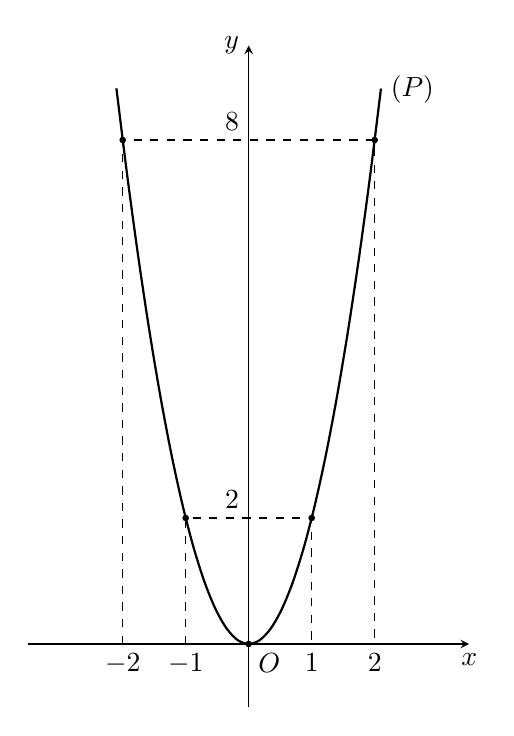
\begin{tikzpicture}[>=stealth, scale=0.8]
\draw[->] (-3.5,0) -- (3.5,0) node[below] {$x$};
\draw[->] (0,-1) -- (0,9.5) node[left] {$y$};
\fill (0,0) circle (1.5pt) node[below right] {$O$};
\draw[domain=-2.1:2.1, smooth, thick] plot (\x, {2*\x*\x});
\draw[dashed] (-2,0) node[below]{$-2$} |- (0,8) node[above left]{$8$} -| (2,0) node[below]{$2$};
\draw[dashed] (-1,0) node[below]{$-1$} |- (0,2) node[above left]{$2$} -| (1,0) node[below]{$1$};
\fill (-2,8) circle (1.5pt); \fill (2,8) circle (1.5pt);
\fill (-1,2) circle (1.5pt); \fill (1,2) circle (1.5pt);
\node[right] at (2.1, 8.8) {$(P)$};
\end{tikzpicture}
\end{center}
\textbf{b)} Kiểm tra các điểm $C(3; 18)$ và $D(-2; 10)$ \hfill \textit{(0,5 điểm)} \par
Xét điểm $C(3; 18)$, thay $x = 3$ vào hàm số của $(P)$, ta được:
$$ y = 2 \cdot 3^2 = 2 \cdot 9 = 18 $$
Giá trị này bằng với tung độ của điểm $C$ nên điểm $C(3; 18)$ thuộc $(P)$. \par
Xét điểm $D(-2; 10)$, thay $x = -2$ vào hàm số của $(P)$, ta được:
$$ y = 2 \cdot (-2)^2 = 2 \cdot 4 = 8 $$
Giá trị này khác với tung độ của điểm $D$ ($8 \neq 10$) nên điểm $D(-2; 10)$ không thuộc $(P)$. \par
Vậy điểm $C(3; 18)$ thuộc $(P)$ và điểm $D(-2; 10)$ không thuộc $(P)$.
}
\end{bt}

\begin{bt}%[9D6H18-2]%[ma:fd442b83]
% nguon: Tuyển tập đề thi Tuyển sinh 10 TP.HCM
Cho parabol $(P): y = \frac{1}{2}x^2$.
\textbf{a)} Vẽ đồ thị $(P)$ trên mặt phẳng tọa độ. \par
\textbf{b)} Tìm tọa độ các điểm $M$ thuộc $(P)$ sao cho tung độ của $M$ gấp đôi hoành độ.
\loigiai{
\textbf{a)} Vẽ đồ thị $(P)$ \hfill \textit{(1,0 điểm)} \par
Bảng giá trị:
\begin{center}
\begin{tabular}{|c|c|c|c|c|c|}
\hline
$x$ & $-4$ & $-2$ & $0$ & $2$ & $4$ \\
\hline
$y = \frac{1}{2}x^2$ & $8$ & $2$ & $0$ & $2$ & $8$ \\
\hline
\end{tabular}
\end{center}
Đồ thị hàm số $(P)$ là đường parabol đi qua gốc tọa độ $O$, nhận trục $Oy$ làm trục đối xứng và nằm phía trên trục hoành.
\begin{center}
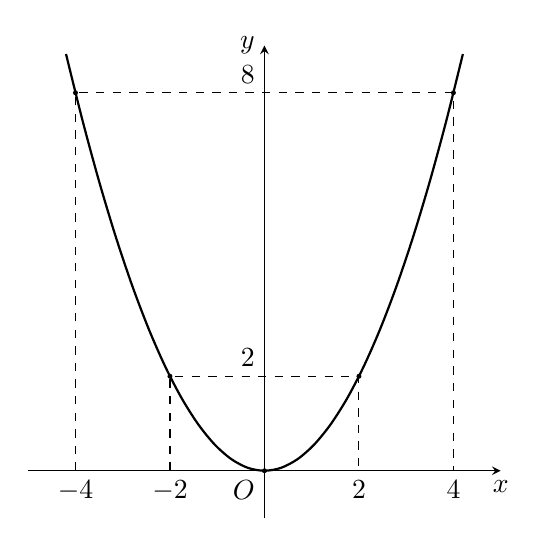
\begin{tikzpicture}[>=stealth, scale=0.6]
\draw[->] (-5,0) -- (5,0) node[below] {$x$};
\draw[->] (0,-1) -- (0,9) node[left] {$y$};
\fill (0,0) circle (1.5pt) node[below left] {$O$};
\draw[domain=-4.2:4.2, smooth, thick] plot (\x, {0.5*\x*\x});
\draw[dashed] (-4,0) node[below]{$-4$} |- (0,8) node[above left]{$8$} -| (4,0) node[below]{$4$};
\draw[dashed] (-2,0) node[below]{$-2$} |- (0,2) node[above left]{$2$} -| (2,0) node[below]{$2$};
\fill (-4,8) circle (1.5pt); \fill (4,8) circle (1.5pt);
\fill (-2,2) circle (1.5pt); \fill (2,2) circle (1.5pt);
\end{tikzpicture}
\end{center}
\textbf{b)} Tìm tọa độ các điểm $M$ \hfill \textit{(0,5 điểm)} \par
Gọi tọa độ điểm $M$ là $(x_M; y_M)$. Vì $M$ thuộc $(P)$ nên $y_M = \frac{1}{2}x_M^2$. \par
Theo đề bài, tung độ gấp đôi hoành độ nên ta có phương trình:
$$ \frac{1}{2}x_M^2 = 2x_M $$
$$ \Leftrightarrow x_M^2 - 4x_M = 0 $$
$$ \Leftrightarrow x_M(x_M - 4) = 0 $$
$$ \Leftrightarrow \heva{&x_M = 0 \\ &x_M = 4} $$
Với $x_M = 0 \Rightarrow y_M = 0$, ta được điểm $M_1(0; 0)$[cite: 1]. \par
Với $x_M = 4 \Rightarrow y_M = 8$, ta được điểm $M_2(4; 8)$. \par
Vậy tọa độ các điểm cần tìm là $(0; 0)$ và $(4; 8)$.
}
\end{bt}

\begin{bt}%[9D6H18-2]%[ma:b8626379]
% nguon: Tuyển tập đề thi Tuyển sinh 10 TP.HCM
Cho hàm số $y = -\frac{1}{2}x^2$ có đồ thị là $(P)$.
\textbf{a)} Vẽ đồ thị $(P)$ trên hệ trục tọa độ. \par
\textbf{b)} Tìm các điểm $A$ thuộc đồ thị $(P)$ sao cho hoành độ và tung độ của điểm đó là hai số đối nhau.
\loigiai{
\textbf{a)} Vẽ đồ thị $(P)$ \hfill \textit{(1,0 điểm)} \par
Bảng giá trị:
\begin{center}
\begin{tabular}{|c|c|c|c|c|c|}
\hline
$x$ & $-4$ & $-2$ & $0$ & $2$ & $4$ \\
\hline
$y = -\frac{1}{2}x^2$ & $-8$ & $-2$ & $0$ & $-2$ & $-8$ \\
\hline
\end{tabular}
\end{center}
Đồ thị hàm số $(P)$ là đường parabol đi qua gốc tọa độ $O$, nhận trục $Oy$ làm trục đối xứng và nằm phía dưới trục hoành.
\begin{center}
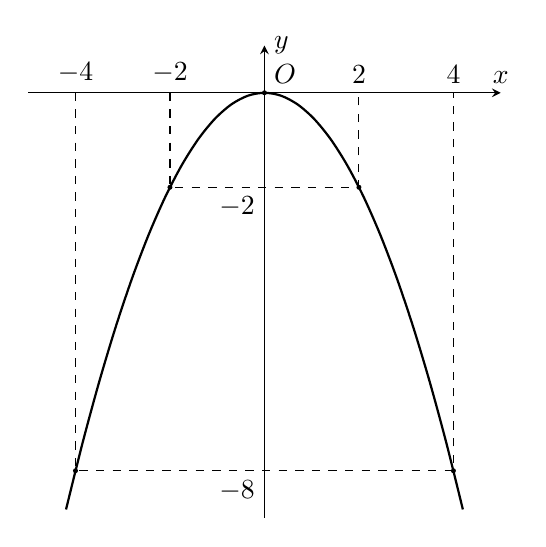
\begin{tikzpicture}[>=stealth, scale=0.6]
\draw[->] (-5,0) -- (5,0) node[above] {$x$};
\draw[->] (0,-9) -- (0,1) node[right] {$y$};
\fill (0,0) circle (1.5pt) node[above right] {$O$};
\draw[domain=-4.2:4.2, smooth, thick] plot (\x, {-0.5*\x*\x});
\draw[dashed] (-4,0) node[above]{$-4$} |- (0,-8) node[below left]{$-8$} -| (4,0) node[above]{$4$};
\draw[dashed] (-2,0) node[above]{$-2$} |- (0,-2) node[below left]{$-2$} -| (2,0) node[above]{$2$};
\fill (-4,-8) circle (1.5pt); \fill (4,-8) circle (1.5pt);
\fill (-2,-2) circle (1.5pt); \fill (2,-2) circle (1.5pt);
\end{tikzpicture}
\end{center}
\textbf{b)} Tìm các điểm $A$ \hfill \textit{(0,5 điểm)} \par
Gọi tọa độ điểm $A$ là $(x_A; y_A)$. Vì $A \in (P)$ nên $y_A = -\frac{1}{2}x_A^2$. \par
Theo đề bài, hoành độ và tung độ là hai số đối nhau nên $y_A = -x_A$. \par
Ta có phương trình:
$$ -\frac{1}{2}x_A^2 = -x_A $$
$$ \Leftrightarrow x_A^2 - 2x_A = 0 $$
$$ \Leftrightarrow x_A(x_A - 2) = 0 $$
$$ \Leftrightarrow \heva{&x_A = 0 \\ &x_A = 2} $$
Với $x_A = 0 \Rightarrow y_A = 0$, ta được điểm $A_1(0; 0)$[cite: 1, 10]. \par
Với $x_A = 2 \Rightarrow y_A = -2$, ta được điểm $A_2(2; -2)$. \par
Vậy tọa độ các điểm cần tìm là $(0; 0)$ và $(2; -2)$.
}
\end{bt}

\begin{bt}%[9D6H18-2]%[ma:e2995c57]
% nguon: Tuyển tập đề thi Tuyển sinh 10 TP.HCM
Cho parabol $(P): y = -2x^2$.
\textbf{a)} Vẽ đồ thị $(P)$ trên hệ trục tọa độ. \par
\textbf{b)} Tìm các điểm thuộc đồ thị $(P)$ có tung độ bằng $-8$.
\loigiai{
\textbf{a)} Vẽ đồ thị $(P)$ \hfill \textit{(1,0 điểm)} \par
Bảng giá trị:
\begin{center}
\begin{tabular}{|c|c|c|c|c|c|}
\hline
$x$ & $-2$ & $-1$ & $0$ & $1$ & $2$ \\
\hline
$y = -2x^2$ & $-8$ & $-2$ & $0$ & $-2$ & $-8$ \\
\hline
\end{tabular}
\end{center}
Đồ thị hàm số $(P)$ là đường parabol đi qua gốc tọa độ $O$, nhận trục $Oy$ làm trục đối xứng và nằm phía dưới trục hoành.
\begin{center}
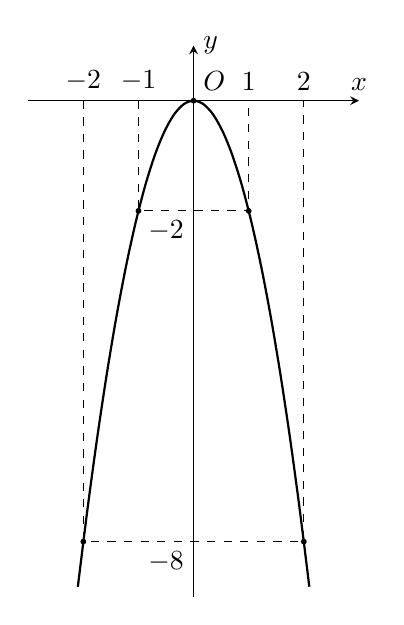
\begin{tikzpicture}[>=stealth, scale=0.7]
\draw[->] (-3,0) -- (3,0) node[above] {$x$};
\draw[->] (0,-9) -- (0,1) node[right] {$y$};
\fill (0,0) circle (1.5pt) node[above right] {$O$};
\draw[domain=-2.1:2.1, smooth, thick] plot (\x, {-2*\x*\x});
\draw[dashed] (-2,0) node[above]{$-2$} |- (0,-8) node[below left]{$-8$} -| (2,0) node[above]{$2$};
\draw[dashed] (-1,0) node[above]{$-1$} |- (0,-2) node[below left]{$-2$} -| (1,0) node[above]{$1$};
\fill (-2,-8) circle (1.5pt); \fill (2,-8) circle (1.5pt);
\fill (-1,-2) circle (1.5pt); \fill (1,-2) circle (1.5pt);
\end{tikzpicture}
\end{center}
\textbf{b)} Tìm các điểm thuộc $(P)$ \hfill \textit{(0,5 điểm)} \par
Gọi điểm cần tìm là $M(x_M; y_M)$. Vì $M \in (P)$ và có tung độ $y_M = -8$ nên ta có phương trình:
$$ -2x_M^2 = -8 $$
$$ \Leftrightarrow x_M^2 = 4 $$
$$ \Leftrightarrow x_M = 2 \text{ hoặc } x_M = -2 $$
Với $x_M = 2$, ta được điểm $(2; -8)$. \par
Với $x_M = -2$, ta được điểm $(-2; -8)$. \par
Vậy có hai điểm thỏa mãn yêu cầu bài toán là $(2; -8)$ và $(-2; -8)$[cite: 1, 34].
}
\end{bt}

\begin{bt}%[9D6H18-2]%[ma:c5303a6d]
% nguon: Tuyển tập đề thi Tuyển sinh 10 TP.HCM
Cho hàm số $y = \frac{1}{4}x^2$ có đồ thị là $(P)$.
\textbf{a)} Vẽ $(P)$ trên hệ trục tọa độ. \par
\textbf{b)} Tìm các điểm trên $(P)$ (khác gốc tọa độ) cách đều hai trục tọa độ.
\loigiai{
\textbf{a)} Vẽ đồ thị $(P)$ \hfill \textit{(1,0 điểm)} \par
Bảng giá trị:
\begin{center}
\begin{tabular}{|c|c|c|c|c|c|}
\hline
$x$ & $-4$ & $-2$ & $0$ & $2$ & $4$ \\
\hline
$y = \frac{1}{4}x^2$ & $4$ & $1$ & $0$ & $1$ & $4$ \\
\hline
\end{tabular}
\end{center}
Đồ thị hàm số $(P)$ là đường parabol đi qua gốc tọa độ $O$, nhận trục $Oy$ làm trục đối xứng và nằm phía trên trục hoành.
\begin{center}
\begin{tikzpicture}[>=stealth, scale=0.8]
\draw[->] (-5,0) -- (5,0) node[below] {$x$};
\draw[->] (0,-1) -- (0,5) node[left] {$y$};
\fill (0,0) circle (1.5pt) node[below left] {$O$};
\draw[domain=-4.2:4.2, smooth, thick] plot (\x, {0.25*\x*\x});
\draw[dashed] (-4,0) node[below]{$-4$} |- (0,4) node[above left]{$4$} -| (4,0) node[below]{$4$};
\draw[dashed] (-2,0) node[below]{$-2$} |- (0,1) node[above left]{$1$} -| (2,0) node[below]{$2$};
\fill (-4,4) circle (1.5pt); \fill (4,4) circle (1.5pt);
\fill (-2,1) circle (1.5pt); \fill (2,1) circle (1.5pt);
\end{tikzpicture}
\end{center}
\textbf{b)} Tìm các điểm cách đều hai trục tọa độ \hfill \textit{(0,5 điểm)} \par
Gọi tọa độ điểm cần tìm là $B(x_B; y_B)$. Vì $B \in (P)$ nên $y_B = \frac{1}{4}x_B^2$. \par
Vì điểm $B$ cách đều hai trục tọa độ nên $|x_B| = |y_B|$[cite: 33]. \par
Trường hợp 1: $y_B = x_B$
$$ \frac{1}{4}x_B^2 = x_B \Leftrightarrow x_B^2 - 4x_B = 0 \Leftrightarrow \heva{&x_B = 0 \\ &x_B = 4} $$
Do $B$ khác gốc tọa độ nên nhận $x_B = 4 \Rightarrow y_B = 4$. Ta được điểm $B_1(4; 4)$[cite: 33]. \par
Trường hợp 2: $y_B = -x_B$
$$ \frac{1}{4}x_B^2 = -x_B \Leftrightarrow x_B^2 + 4x_B = 0 \Leftrightarrow \heva{&x_B = 0 \\ &x_B = -4} $$
Do $B$ khác gốc tọa độ nên nhận $x_B = -4 \Rightarrow y_B = 4$. Ta được điểm $B_2(-4; 4)$[cite: 33]. \par
Vậy các điểm cần tìm là $(4; 4)$ và $(-4; 4)$.
}
\end{bt}

\begin{bt}%[9D6H18-2]%[ma:a731a6a9]
% nguon: Tuyển tập đề thi Tuyển sinh 10 TP.HCM
Cho hàm số $y = 2x^2$ có đồ thị là parabol $(P)$.
\textbf{a)} Vẽ đồ thị $(P)$ trên mặt phẳng tọa độ $Oxy$. \par
\textbf{b)} Tìm tọa độ những điểm thuộc $(P)$ có tung độ bằng $18$.
\loigiai{
\textbf{a)} Vẽ đồ thị $(P)$ \hfill \textit{(1,0 điểm)} \par
Bảng giá trị:
\begin{center}
\begin{tabular}{|c|c|c|c|c|c|}
\hline
$x$ & $-2$ & $-1$ & $0$ & $1$ & $2$ \\
\hline
$y = 2x^2$ & $8$ & $2$ & $0$ & $2$ & $8$ \\
\hline
\end{tabular}
\end{center}
Đồ thị hàm số $(P)$ là đường parabol đi qua gốc tọa độ $O$, nhận trục $Oy$ làm trục đối xứng và nằm phía trên trục hoành.
\begin{center}
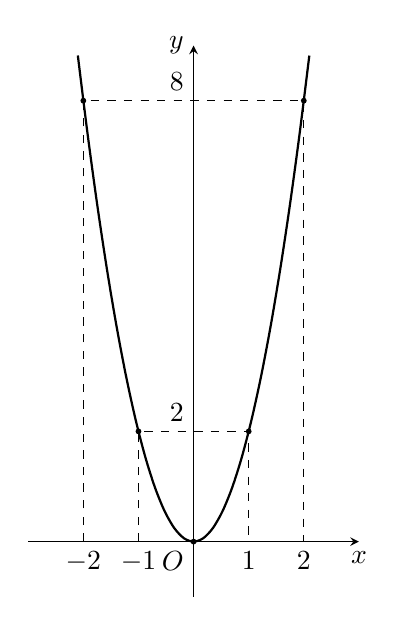
\begin{tikzpicture}[>=stealth, scale=0.7]
\draw[->] (-3,0) -- (3,0) node[below] {$x$};
\draw[->] (0,-1) -- (0,9) node[left] {$y$};
\fill (0,0) circle (1.5pt) node[below left] {$O$};
\draw[domain=-2.1:2.1, smooth, thick] plot (\x, {2*\x*\x});
\draw[dashed] (-2,0) node[below]{$-2$} |- (0,8) node[above left]{$8$} -| (2,0) node[below]{$2$};
\draw[dashed] (-1,0) node[below]{$-1$} |- (0,2) node[above left]{$2$} -| (1,0) node[below]{$1$};
\fill (-2,8) circle (1.5pt); \fill (2,8) circle (1.5pt);
\fill (-1,2) circle (1.5pt); \fill (1,2) circle (1.5pt);
\end{tikzpicture}
\end{center}
\textbf{b)} Tìm các điểm thuộc $(P)$ \hfill \textit{(0,5 điểm)} \par
Gọi điểm cần tìm là $C(x_C; y_C)$. Vì $C \in (P)$ và có tung độ $y_C = 18$ nên ta có phương trình:
$$ 2x_C^2 = 18 $$
$$ \Leftrightarrow x_C^2 = 9 $$
$$ \Leftrightarrow x_C = 3 \text{ hoặc } x_C = -3 $$
Với $x_C = 3$, ta được điểm $(3; 18)$. \par
Với $x_C = -3$, ta được điểm $(-3; 18)$. \par
Vậy tọa độ những điểm cần tìm là $(3; 18)$ và $(-3; 18)$[cite: 1, 12].
}
\end{bt}

\begin{bt}%[9D6H18-2]%[ma:49523185]
% nguon: Tuyển tập đề thi Tuyển sinh 10 TP.HCM
Cho parabol $(P): y = x^2$.
\textbf{a)} Vẽ đồ thị $(P)$ trên hệ trục tọa độ. \par
\textbf{b)} Tìm tọa độ những điểm thuộc $(P)$ có tung độ và hoành độ bằng nhau.
\loigiai{
\textbf{a)} Vẽ đồ thị $(P)$ \hfill \textit{(1,0 điểm)} \par
Bảng giá trị:
\begin{center}
\begin{tabular}{|c|c|c|c|c|c|}
\hline
$x$ & $-2$ & $-1$ & $0$ & $1$ & $2$ \\
\hline
$y = x^2$ & $4$ & $1$ & $0$ & $1$ & $4$ \\
\hline
\end{tabular}
\end{center}
Đồ thị hàm số $(P)$ là đường parabol đi qua gốc tọa độ $O$, nhận trục $Oy$ làm trục đối xứng và nằm phía trên trục hoành.
\begin{center}
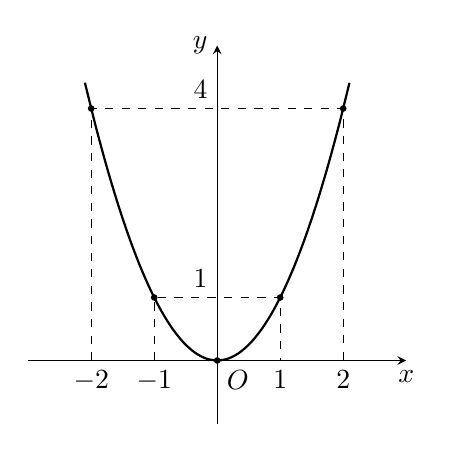
\begin{tikzpicture}[>=stealth, scale=0.8]
\draw[->] (-3,0) -- (3,0) node[below] {$x$};
\draw[->] (0,-1) -- (0,5) node[left] {$y$};
\fill (0,0) circle (1.5pt) node[below right] {$O$};
\draw[domain=-2.1:2.1, smooth, thick] plot (\x, {\x*\x});
\draw[dashed] (-2,0) node[below]{$-2$} |- (0,4) node[above left]{$4$} -| (2,0) node[below]{$2$};
\draw[dashed] (-1,0) node[below]{$-1$} |- (0,1) node[above left]{$1$} -| (1,0) node[below]{$1$};
\fill (-2,4) circle (1.5pt); \fill (2,4) circle (1.5pt);
\fill (-1,1) circle (1.5pt); \fill (1,1) circle (1.5pt);
\end{tikzpicture}
\end{center}
\textbf{b)} Tìm tọa độ các điểm \hfill \textit{(0,5 điểm)} \par
Gọi tọa độ điểm cần tìm là $D(x_D; y_D)$. Vì $D$ thuộc $(P)$ nên $y_D = x_D^2$. \par
Theo đề bài, tung độ và hoành độ bằng nhau nên $y_D = x_D$. \par
Ta có phương trình:
$$ x_D^2 = x_D $$
$$ \Leftrightarrow x_D^2 - x_D = 0 $$
$$ \Leftrightarrow x_D(x_D - 1) = 0 $$
$$ \Leftrightarrow \heva{&x_D = 0 \\ &x_D = 1} $$
Với $x_D = 0 \Rightarrow y_D = 0$, ta được điểm $D_1(0; 0)$[cite: 16]. \par
Với $x_D = 1 \Rightarrow y_D = 1$, ta được điểm $D_2(1; 1)$[cite: 16]. \par
Vậy tọa độ những điểm cần tìm là $(0; 0)$ và $(1; 1)$.
}
\end{bt}

\begin{bt}%[9D6H18-2]%[ma:414ff1a3]
% nguon: Tuyển tập đề thi Tuyển sinh 10 TP.HCM
Cho đồ thị hàm số $y = -\frac{1}{4}x^2$ có đồ thị là $(P)$.
\textbf{a)} Vẽ $(P)$ trên hệ trục tọa độ. \par
\textbf{b)} Tìm các điểm trên $(P)$ có tung độ bằng $-36$.
\loigiai{
\textbf{a)} Vẽ đồ thị $(P)$ \hfill \textit{(1,0 điểm)} \par
Bảng giá trị:
\begin{center}
\begin{tabular}{|c|c|c|c|c|c|}
\hline
$x$ & $-4$ & $-2$ & $0$ & $2$ & $4$ \\
\hline
$y = -\frac{1}{4}x^2$ & $-4$ & $-1$ & $0$ & $-1$ & $-4$ \\
\hline
\end{tabular}
\end{center}
Đồ thị hàm số $(P)$ là đường parabol đi qua gốc tọa độ $O$, nhận trục $Oy$ làm trục đối xứng và nằm phía dưới trục hoành.
\begin{center}
\begin{tikzpicture}[>=stealth, scale=0.8]
\draw[->] (-5,0) -- (5,0) node[above] {$x$};
\draw[->] (0,-5) -- (0,1) node[right] {$y$};
\fill (0,0) circle (1.5pt) node[above right] {$O$};
\draw[domain=-4.2:4.2, smooth, thick] plot (\x, {-0.25*\x*\x});
\draw[dashed] (-4,0) node[above]{$-4$} |- (0,-4) node[below left]{$-4$} -| (4,0) node[above]{$4$};
\draw[dashed] (-2,0) node[above]{$-2$} |- (0,-1) node[below left]{$-1$} -| (2,0) node[above]{$2$};
\fill (-4,-4) circle (1.5pt); \fill (4,-4) circle (1.5pt);
\fill (-2,-1) circle (1.5pt); \fill (2,-1) circle (1.5pt);
\end{tikzpicture}
\end{center}
\textbf{b)} Tìm các điểm trên $(P)$ \hfill \textit{(0,5 điểm)} \par
Gọi điểm cần tìm là $E(x_E; y_E)$. Vì $E \in (P)$ và có tung độ $y_E = -36$ nên ta có phương trình:
$$ -\frac{1}{4}x_E^2 = -36 $$
$$ \Leftrightarrow x_E^2 = 144 $$
$$ \Leftrightarrow x_E = 12 \text{ hoặc } x_E = -12 $$
Với $x_E = 12$, ta có điểm $E_1(12; -36)$[cite: 47]. \par
Với $x_E = -12$, ta có điểm $E_2(-12; -36)$[cite: 47]. \par
Vậy có hai điểm trên $(P)$ thỏa mãn yêu cầu là $(12; -36)$ và $(-12; -36)$.
}
\end{bt}

\begin{bt}%[9D6H18-2]%[ma:8e4727d0]
% nguon: Tuyển tập đề thi Tuyển sinh 10 TP.HCM
Cho parabol $(P): y = \frac{x^2}{4}$.
\textbf{a)} Vẽ đồ thị $(P)$ của hàm số trên. \par
\textbf{b)} Tìm những điểm thuộc $(P)$ sao cho tung độ gấp $4$ lần hoành độ.
\loigiai{
\textbf{a)} Vẽ đồ thị $(P)$ \hfill \textit{(1,0 điểm)} \par
Bảng giá trị:
\begin{center}
\begin{tabular}{|c|c|c|c|c|c|}
\hline
$x$ & $-4$ & $-2$ & $0$ & $2$ & $4$ \\
\hline
$y = \frac{x^2}{4}$ & $4$ & $1$ & $0$ & $1$ & $4$ \\
\hline
\end{tabular}
\end{center}
Đồ thị hàm số $(P)$ là đường parabol đi qua gốc tọa độ $O$, nhận trục $Oy$ làm trục đối xứng và nằm phía trên trục hoành.
\begin{center}
\begin{tikzpicture}[>=stealth, scale=0.8]
\draw[->] (-5,0) -- (5,0) node[below] {$x$};
\draw[->] (0,-1) -- (0,5) node[left] {$y$};
\fill (0,0) circle (1.5pt) node[below left] {$O$};
\draw[domain=-4.2:4.2, smooth, thick] plot (\x, {0.25*\x*\x});
\draw[dashed] (-4,0) node[below]{$-4$} |- (0,4) node[above left]{$4$} -| (4,0) node[below]{$4$};
\draw[dashed] (-2,0) node[below]{$-2$} |- (0,1) node[above left]{$1$} -| (2,0) node[below]{$2$};
\fill (-4,4) circle (1.5pt); \fill (4,4) circle (1.5pt);
\fill (-2,1) circle (1.5pt); \fill (2,1) circle (1.5pt);
\end{tikzpicture}
\end{center}
\textbf{b)} Tìm những điểm thuộc $(P)$ \hfill \textit{(0,5 điểm)} \par
Gọi điểm cần tìm là $F(x_F; y_F)$. Vì $F \in (P)$ nên $y_F = \frac{1}{4}x_F^2$. \par
Theo đề bài, tung độ gấp $4$ lần hoành độ nên $y_F = 4x_F$[cite: 1, 24]. \par
Ta có phương trình:
$$ \frac{1}{4}x_F^2 = 4x_F $$
$$ \Leftrightarrow x_F^2 - 16x_F = 0 $$
$$ \Leftrightarrow x_F(x_F - 16) = 0 $$
$$ \Leftrightarrow \heva{&x_F = 0 \\ &x_F = 16} $$
Với $x_F = 0 \Rightarrow y_F = 0$, ta được điểm $F_1(0; 0)$. \par
Với $x_F = 16 \Rightarrow y_F = 4(16) = 64$, ta được điểm $F_2(16; 64)$. \par
Vậy tọa độ những điểm cần tìm là $(0; 0)$ và $(16; 64)$.
}
\end{bt}

\begin{bt}%[9D6H18-2]%[ma:6020ba7e]
% nguon: Tuyển tập đề thi Tuyển sinh 10 TP.HCM
Cho hàm số $y = -\frac{x^2}{2}$ có đồ thị là $(P)$.
\textbf{a)} Vẽ đồ thị $(P)$ trên hệ trục tọa độ. \par
\textbf{b)} Tìm tọa độ điểm $A$ thuộc $(P)$ có tung độ bằng $-2$.
\loigiai{
\textbf{a)} Vẽ đồ thị $(P)$ \hfill \textit{(1,0 điểm)} \par
Bảng giá trị:
\begin{center}
\begin{tabular}{|c|c|c|c|c|c|}
\hline
$x$ & $-4$ & $-2$ & $0$ & $2$ & $4$ \\
\hline
$y = -\frac{x^2}{2}$ & $-8$ & $-2$ & $0$ & $-2$ & $-8$ \\
\hline
\end{tabular}
\end{center}
Đồ thị hàm số $(P)$ là đường parabol đi qua gốc tọa độ $O$, nhận trục $Oy$ làm trục đối xứng và nằm phía dưới trục hoành.
\begin{center}
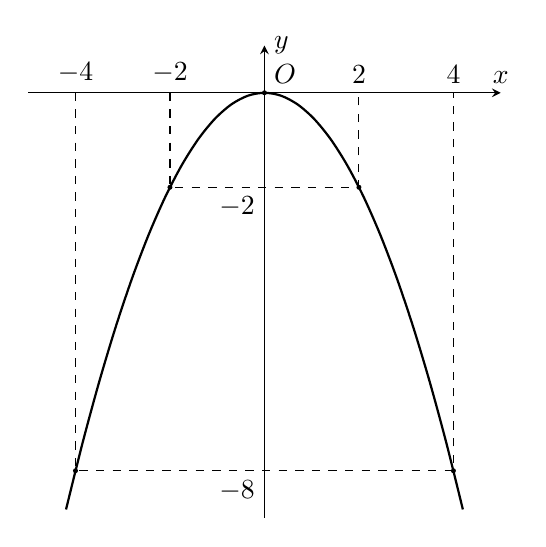
\begin{tikzpicture}[>=stealth, scale=0.6]
\draw[->] (-5,0) -- (5,0) node[above] {$x$};
\draw[->] (0,-9) -- (0,1) node[right] {$y$};
\fill (0,0) circle (1.5pt) node[above right] {$O$};
\draw[domain=-4.2:4.2, smooth, thick] plot (\x, {-0.5*\x*\x});
\draw[dashed] (-4,0) node[above]{$-4$} |- (0,-8) node[below left]{$-8$} -| (4,0) node[above]{$4$};
\draw[dashed] (-2,0) node[above]{$-2$} |- (0,-2) node[below left]{$-2$} -| (2,0) node[above]{$2$};
\fill (-4,-8) circle (1.5pt); \fill (4,-8) circle (1.5pt);
\fill (-2,-2) circle (1.5pt); \fill (2,-2) circle (1.5pt);
\end{tikzpicture}
\end{center}
\textbf{b)} Tìm tọa độ điểm $A$ \hfill \textit{(0,5 điểm)} \par
Vì điểm $A$ thuộc $(P)$ và có tung độ bằng $-2$ nên ta thay $y = -2$ vào phương trình hàm số:
$$ -2 = -\frac{x^2}{2} $$
$$ \Leftrightarrow x^2 = 4 $$
$$ \Leftrightarrow x = 2 \text{ hoặc } x = -2 $$
Với $x = 2$, ta được điểm $(2; -2)$. \par
Với $x = -2$, ta được điểm $(-2; -2)$. \par
Vậy tọa độ các điểm $A$ cần tìm là $(2; -2)$ và $(-2; -2)$[cite: 1].
}
\end{bt}

\begin{bt}%[9D6H18-2]%[ma:43206e52]
% nguon: Tuyển tập đề thi Tuyển sinh 10 TP.HCM
Cho hàm số $y = 2x^2$ có đồ thị là parabol $(P)$.
\textbf{a)} Vẽ $(P)$ trên hệ trục tọa độ. \par
\textbf{b)} Tìm tọa độ các điểm $K$ thuộc $(P)$ có hoành độ bằng hai lần tung độ.
\loigiai{
\textbf{a)} Vẽ đồ thị $(P)$ \hfill \textit{(1,0 điểm)} \par
Bảng giá trị:
\begin{center}
\begin{tabular}{|c|c|c|c|c|c|}
\hline
$x$ & $-2$ & $-1$ & $0$ & $1$ & $2$ \\
\hline
$y = 2x^2$ & $8$ & $2$ & $0$ & $2$ & $8$ \\
\hline
\end{tabular}
\end{center}
Đồ thị hàm số $(P)$ là đường parabol đi qua gốc tọa độ $O$, nhận trục $Oy$ làm trục đối xứng và nằm phía trên trục hoành.
\begin{center}
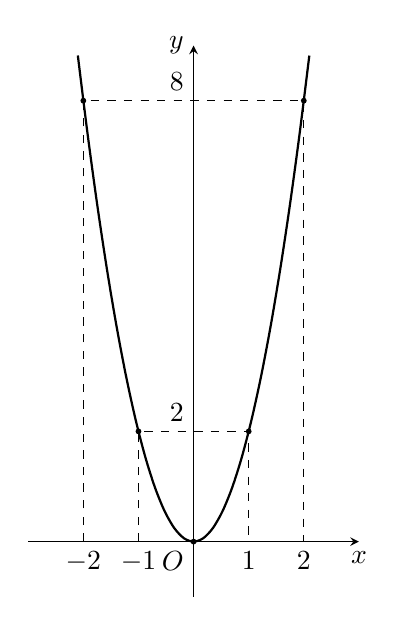
\begin{tikzpicture}[>=stealth, scale=0.7]
\draw[->] (-3,0) -- (3,0) node[below] {$x$};
\draw[->] (0,-1) -- (0,9) node[left] {$y$};
\fill (0,0) circle (1.5pt) node[below left] {$O$};
\draw[domain=-2.1:2.1, smooth, thick] plot (\x, {2*\x*\x});
\draw[dashed] (-2,0) node[below]{$-2$} |- (0,8) node[above left]{$8$} -| (2,0) node[below]{$2$};
\draw[dashed] (-1,0) node[below]{$-1$} |- (0,2) node[above left]{$2$} -| (1,0) node[below]{$1$};
\fill (-2,8) circle (1.5pt); \fill (2,8) circle (1.5pt);
\fill (-1,2) circle (1.5pt); \fill (1,2) circle (1.5pt);
\end{tikzpicture}
\end{center}
\textbf{b)} Tìm tọa độ các điểm $K$ \hfill \textit{(0,5 điểm)} \par
Gọi tọa độ điểm $K$ là $(x_K; y_K)$. Vì $K \in (P)$ nên $y_K = 2x_K^2$. \par
Theo đề bài, hoành độ bằng hai lần tung độ nên $x_K = 2y_K$[cite: 36]. \par
Ta có phương trình:
$$ x_K = 2(2x_K^2) $$
$$ \Leftrightarrow 4x_K^2 - x_K = 0 $$
$$ \Leftrightarrow x_K(4x_K - 1) = 0 $$
$$ \Leftrightarrow \heva{&x_K = 0 \\ &x_K = \frac{1}{4}} $$
Với $x_K = 0 \Rightarrow y_K = 0$, ta được điểm $K_1(0; 0)$[cite: 36]. \par
Với $x_K = \frac{1}{4} \Rightarrow y_K = 2\left(\frac{1}{4}\right)^2 = 2 \cdot \frac{1}{16} = \frac{1}{8}$. \par
(Kiểm tra lại: $x_K = 2y_K \Leftrightarrow \frac{1}{4} = 2 \cdot \frac{1}{8}$ đúng). \par
Ta được điểm $K_2\left(\frac{1}{4}; \frac{1}{8}\right)$. \par
Vậy tọa độ các điểm cần tìm là $(0; 0)$ và $\left(\frac{1}{4}; \frac{1}{8}\right)$[cite: 36].
}
\end{bt}

\begin{bt}%[9D6H18-2]%[ma:4db76812]
% nguon: Tuyển tập đề thi Tuyển sinh 10 TP.HCM
Cho parabol $(P): y = x^2$.
\textbf{a)} Vẽ đồ thị $(P)$ trên mặt phẳng tọa độ. \par
\textbf{b)} Tìm tọa độ các điểm $A$ thuộc $(P)$ sao cho tổng hoành độ và tung độ của điểm đó bằng $6$.
\loigiai{
\textbf{a)} Vẽ đồ thị $(P): y = x^2$ \hfill \textit{(1,0 điểm)} \par
Bảng giá trị:
\begin{center}
\begin{tabular}{|c|c|c|c|c|c|}
\hline
$x$ & $-2$ & $-1$ & $0$ & $1$ & $2$ \\
\hline
$y = x^2$ & $4$ & $1$ & $0$ & $1$ & $4$ \\
\hline
\end{tabular}
\end{center}
Đồ thị hàm số $(P)$ là một đường parabol đi qua gốc tọa độ $O$, nhận trục $Oy$ làm trục đối xứng và nằm phía trên trục hoành.
\begin{center}
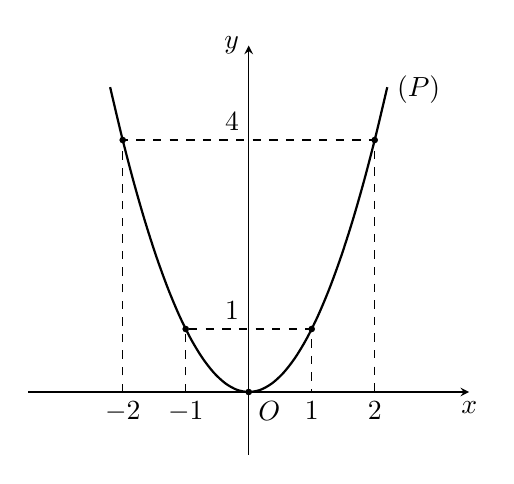
\begin{tikzpicture}[>=stealth, scale=0.8]
\draw[->] (-3.5,0) -- (3.5,0) node[below] {$x$};
\draw[->] (0,-1) -- (0,5.5) node[left] {$y$};
\fill (0,0) circle (1.5pt) node[below right] {$O$};
\draw[domain=-2.2:2.2, smooth, thick] plot (\x, {\x*\x});
\draw[dashed] (-2,0) node[below]{$-2$} |- (0,4) node[above left]{$4$} -| (2,0) node[below]{$2$};
\draw[dashed] (-1,0) node[below]{$-1$} |- (0,1) node[above left]{$1$} -| (1,0) node[below]{$1$};
\fill (-2,4) circle (1.5pt); \fill (2,4) circle (1.5pt);
\fill (-1,1) circle (1.5pt); \fill (1,1) circle (1.5pt);
\node[right] at (2.2, 4.8) {$(P)$};
\end{tikzpicture}
\end{center}
\textbf{b)} Tìm tọa độ các điểm $A$ \hfill \textit{(0,5 điểm)} \par
Gọi tọa độ điểm $A$ là $(x_A; y_A)$. Vì $A \in (P)$ nên $y_A = x_A^2$. \par
Theo đề bài, tổng hoành độ và tung độ bằng $6$, ta có phương trình:
$$ x_A + y_A = 6 $$
$$ \Leftrightarrow x_A + x_A^2 = 6 $$
$$ \Leftrightarrow x_A^2 + x_A - 6 = 0 $$
$$ \Leftrightarrow (x_A - 2)(x_A + 3) = 0 $$
$$ \Leftrightarrow \heva{&x_A = 2 \\ &x_A = -3} $$
Với $x_A = 2 \Rightarrow y_A = 2^2 = 4$, ta được điểm $A_1(2; 4)$. \par
Với $x_A = -3 \Rightarrow y_A = (-3)^2 = 9$, ta được điểm $A_2(-3; 9)$. \par
Vậy tọa độ các điểm $A$ cần tìm là $(2; 4)$ và $(-3; 9)$.
}
\end{bt}

\begin{bt}%[9D6H18-3]%[ma:c8ebd171]
% nguon: Tuyển tập đề thi Tuyển sinh 10 TP.HCM
Cho parabol $(P): y = -x^2$ và đường thẳng $(d): y = 3x - 4$.
\textbf{a)} Vẽ đồ thị $(P)$ trên hệ trục tọa độ. \par
\textbf{b)} Tìm tọa độ giao điểm của $(P)$ và $(d)$ bằng phép tính.
\loigiai{
\textbf{a)} Vẽ đồ thị $(P): y = -x^2$ \hfill \textit{(1,0 điểm)} \par
Bảng giá trị:
\begin{center}
\begin{tabular}{|c|c|c|c|c|c|}
\hline
$x$ & $-2$ & $-1$ & $0$ & $1$ & $2$ \\
\hline
$y = -x^2$ & $-4$ & $-1$ & $0$ & $-1$ & $-4$ \\
\hline
\end{tabular}
\end{center}
Đồ thị hàm số $(P)$ là một đường parabol đi qua gốc tọa độ $O$, nhận trục $Oy$ làm trục đối xứng và nằm phía dưới trục hoành.
\begin{center}
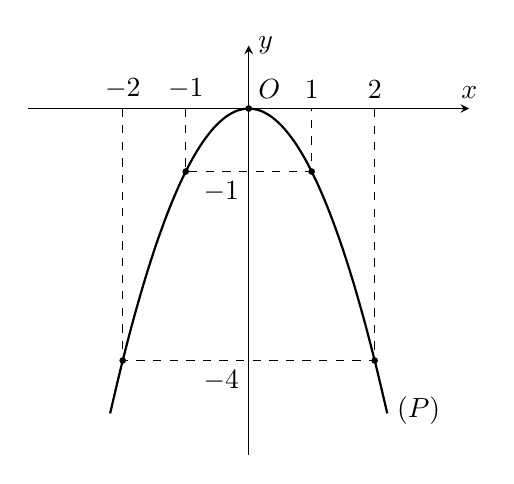
\begin{tikzpicture}[>=stealth, scale=0.8]
\draw[->] (-3.5,0) -- (3.5,0) node[above] {$x$};
\draw[->] (0,-5.5) -- (0,1) node[right] {$y$};
\fill (0,0) circle (1.5pt) node[above right] {$O$};
\draw[domain=-2.2:2.2, smooth, thick] plot (\x, {-\x*\x});
\draw[dashed] (-2,0) node[above]{$-2$} |- (0,-4) node[below left]{$-4$} -| (2,0) node[above]{$2$};
\draw[dashed] (-1,0) node[above]{$-1$} |- (0,-1) node[below left]{$-1$} -| (1,0) node[above]{$1$};
\fill (-2,-4) circle (1.5pt); \fill (2,-4) circle (1.5pt);
\fill (-1,-1) circle (1.5pt); \fill (1,-1) circle (1.5pt);
\node[right] at (2.2, -4.8) {$(P)$};
\end{tikzpicture}
\end{center}
\textbf{b)} Tìm tọa độ giao điểm của $(P)$ và $(d)$ \hfill \textit{(0,5 điểm)} \par
Phương trình hoành độ giao điểm của $(P)$ và $(d)$ là:
$$ -x^2 = 3x - 4 $$
$$ \Leftrightarrow x^2 + 3x - 4 = 0 $$
Vì $a + b + c = 1 + 3 + (-4) = 0$ nên phương trình có hai nghiệm:
$$ x_1 = 1; \quad x_2 = -4 $$
Với $x = 1 \Rightarrow y = -(1)^2 = -1$. Ta được giao điểm thứ nhất là $(1; -1)$. \par
Với $x = -4 \Rightarrow y = -(-4)^2 = -16$. Ta được giao điểm thứ hai là $(-4; -16)$. \par
Vậy tọa độ giao điểm của $(P)$ và $(d)$ là $(1; -1)$ và $(-4; -16)$.
}
\end{bt}

\begin{bt}%[9D6H18-2]%[ma:9fb93691]
% nguon: Tuyển tập đề thi Tuyển sinh 10 TP.HCM
Cho parabol $(P): y = \frac{1}{2}x^2$.
\textbf{a)} Vẽ đồ thị $(P)$ trên hệ trục tọa độ. \par
\textbf{b)} Tìm tọa độ các điểm $B$ thuộc $(P)$ sao cho tung độ lớn hơn hoành độ $4$ đơn vị.
\loigiai{
\textbf{a)} Vẽ đồ thị $(P): y = \frac{1}{2}x^2$ \hfill \textit{(1,0 điểm)} \par
Bảng giá trị:
\begin{center}
\begin{tabular}{|c|c|c|c|c|c|}
\hline
$x$ & $-4$ & $-2$ & $0$ & $2$ & $4$ \\
\hline
$y = \frac{1}{2}x^2$ & $8$ & $2$ & $0$ & $2$ & $8$ \\
\hline
\end{tabular}
\end{center}
Đồ thị hàm số $(P)$ là một đường parabol đi qua gốc tọa độ $O$, nhận trục $Oy$ làm trục đối xứng và nằm phía trên trục hoành.
\begin{center}
\begin{tikzpicture}[>=stealth, scale=0.7]
\draw[->] (-5.5,0) -- (5.5,0) node[below] {$x$};
\draw[->] (0,-1) -- (0,9.5) node[left] {$y$};
\fill (0,0) circle (1.5pt) node[below right] {$O$};
\draw[domain=-4.2:4.2, smooth, thick] plot (\x, {0.5*\x*\x});
\draw[dashed] (-4,0) node[below]{$-4$} |- (0,8) node[above left]{$8$} -| (4,0) node[below]{$4$};
\draw[dashed] (-2,0) node[below]{$-2$} |- (0,2) node[above left]{$2$} -| (2,0) node[below]{$2$};
\fill (-4,8) circle (1.5pt); \fill (4,8) circle (1.5pt);
\fill (-2,2) circle (1.5pt); \fill (2,2) circle (1.5pt);
\node[right] at (4.2, 8.8) {$(P)$};
\end{tikzpicture}
\end{center}
\textbf{b)} Tìm tọa độ các điểm $B$ \hfill \textit{(0,5 điểm)} \par
Gọi tọa độ điểm $B$ là $(x_B; y_B)$. Vì $B \in (P)$ nên $y_B = \frac{1}{2}x_B^2$. \par
Theo đề bài, tung độ lớn hơn hoành độ $4$ đơn vị, ta có phương trình:
$$ y_B - x_B = 4 $$
$$ \Leftrightarrow \frac{1}{2}x_B^2 - x_B - 4 = 0 $$
$$ \Leftrightarrow x_B^2 - 2x_B - 8 = 0 $$
$$ \Leftrightarrow (x_B - 4)(x_B + 2) = 0 $$
$$ \Leftrightarrow \heva{&x_B = 4 \\ &x_B = -2} $$
Với $x_B = 4 \Rightarrow y_B = \frac{1}{2} \cdot 4^2 = 8$, ta được điểm $B_1(4; 8)$. \par
Với $x_B = -2 \Rightarrow y_B = \frac{1}{2} \cdot (-2)^2 = 2$, ta được điểm $B_2(-2; 2)$. \par
Vậy tọa độ các điểm $B$ cần tìm là $(4; 8)$ và $(-2; 2)$.
}
\end{bt}

\begin{bt}%[9D6H18-3]%[ma:a40b5424]
% nguon: Tuyển tập đề thi Tuyển sinh 10 TP.HCM
Cho parabol $(P): y = -\frac{1}{4}x^2$ và đường thẳng $(d): y = \frac{1}{2}x - 2$.
\textbf{a)} Vẽ đồ thị $(P)$ trên hệ trục tọa độ. \par
\textbf{b)} Bằng phép tính, tìm tọa độ giao điểm của $(P)$ và $(d)$.
\loigiai{
\textbf{a)} Vẽ đồ thị $(P): y = -\frac{1}{4}x^2$ \hfill \textit{(1,0 điểm)} \par
Bảng giá trị:
\begin{center}
\begin{tabular}{|c|c|c|c|c|c|}
\hline
$x$ & $-4$ & $-2$ & $0$ & $2$ & $4$ \\
\hline
$y = -\frac{1}{4}x^2$ & $-4$ & $-1$ & $0$ & $-1$ & $-4$ \\
\hline
\end{tabular}
\end{center}
Đồ thị hàm số $(P)$ là một đường parabol đi qua gốc tọa độ $O$, nhận trục $Oy$ làm trục đối xứng và nằm phía dưới trục hoành.
\begin{center}
\begin{tikzpicture}[>=stealth, scale=0.8]
\draw[->] (-5.5,0) -- (5.5,0) node[above] {$x$};
\draw[->] (0,-5.5) -- (0,1) node[right] {$y$};
\fill (0,0) circle (1.5pt) node[above right] {$O$};
\draw[domain=-4.5:4.5, smooth, thick] plot (\x, {-0.25*\x*\x});
\draw[dashed] (-4,0) node[above]{$-4$} |- (0,-4) node[below left]{$-4$} -| (4,0) node[above]{$4$};
\draw[dashed] (-2,0) node[above]{$-2$} |- (0,-1) node[below left]{$-1$} -| (2,0) node[above]{$2$};
\fill (-4,-4) circle (1.5pt); \fill (4,-4) circle (1.5pt);
\fill (-2,-1) circle (1.5pt); \fill (2,-1) circle (1.5pt);
\node[right] at (4.5, -5) {$(P)$};
\end{tikzpicture}
\end{center}
\textbf{b)} Tìm tọa độ giao điểm của $(P)$ và $(d)$ \hfill \textit{(0,5 điểm)} \par
Phương trình hoành độ giao điểm của $(P)$ và $(d)$ là:
$$ -\frac{1}{4}x^2 = \frac{1}{2}x - 2 $$
$$ \Leftrightarrow x^2 + 2x - 8 = 0 $$
$$ \Leftrightarrow (x - 2)(x + 4) = 0 $$
$$ \Leftrightarrow \heva{&x = 2 \\ &x = -4} $$
Với $x = 2 \Rightarrow y = -\frac{1}{4}(2)^2 = -1$. Ta được giao điểm thứ nhất là $(2; -1)$. \par
Với $x = -4 \Rightarrow y = -\frac{1}{4}(-4)^2 = -4$. Ta được giao điểm thứ hai là $(-4; -4)$. \par
Vậy tọa độ giao điểm của $(P)$ và $(d)$ là $(2; -1)$ và $(-4; -4)$.
}
\end{bt}

\begin{bt}%[9D6H18-2]%[ma:907b5db8]
% nguon: Tuyển tập đề thi Tuyển sinh 10 TP.HCM
Cho parabol $(P): y = \frac{1}{4}x^2$.
\textbf{a)} Vẽ đồ thị $(P)$ trên mặt phẳng tọa độ. \par
\textbf{b)} Tìm tọa độ các điểm $C$ thuộc $(P)$ (khác gốc tọa độ $O$) sao cho tích của hoành độ và tung độ bằng $2$.
\loigiai{
\textbf{a)} Vẽ đồ thị $(P): y = \frac{1}{4}x^2$ \hfill \textit{(1,0 điểm)} \par
Bảng giá trị:
\begin{center}
\begin{tabular}{|c|c|c|c|c|c|}
\hline
$x$ & $-4$ & $-2$ & $0$ & $2$ & $4$ \\
\hline
$y = \frac{1}{4}x^2$ & $4$ & $1$ & $0$ & $1$ & $4$ \\
\hline
\end{tabular}
\end{center}
Đồ thị hàm số $(P)$ là một đường parabol đi qua gốc tọa độ $O$, nhận trục $Oy$ làm trục đối xứng và nằm phía trên trục hoành.
\begin{center}
\begin{tikzpicture}[>=stealth, scale=0.8]
\draw[->] (-5.5,0) -- (5.5,0) node[below] {$x$};
\draw[->] (0,-1) -- (0,5.5) node[left] {$y$};
\fill (0,0) circle (1.5pt) node[below right] {$O$};
\draw[domain=-4.2:4.2, smooth, thick] plot (\x, {0.25*\x*\x});
\draw[dashed] (-4,0) node[below]{$-4$} |- (0,4) node[above left]{$4$} -| (4,0) node[below]{$4$};
\draw[dashed] (-2,0) node[below]{$-2$} |- (0,1) node[above left]{$1$} -| (2,0) node[below]{$2$};
\fill (-4,4) circle (1.5pt); \fill (4,4) circle (1.5pt);
\fill (-2,1) circle (1.5pt); \fill (2,1) circle (1.5pt);
\node[right] at (4.2, 4.4) {$(P)$};
\end{tikzpicture}
\end{center}
\textbf{b)} Tìm tọa độ các điểm $C$ \hfill \textit{(0,5 điểm)} \par
Gọi tọa độ điểm $C$ là $(x_C; y_C)$. Vì $C \in (P)$ nên $y_C = \frac{1}{4}x_C^2$. \par
Theo đề bài, tích của hoành độ và tung độ bằng $2$, ta có phương trình:
$$ x_C \cdot y_C = 2 $$
$$ \Leftrightarrow x_C \cdot \left(\frac{1}{4}x_C^2\right) = 2 $$
$$ \Leftrightarrow x_C^3 = 8 $$
$$ \Leftrightarrow x_C = 2 $$
Với $x_C = 2 \Rightarrow y_C = \frac{1}{4} \cdot 2^2 = 1$. Ta được điểm $C(2; 1)$. \par
Vậy tọa độ điểm $C$ cần tìm là $(2; 1)$.
}
\end{bt}

\begin{bt}%[9D6H18-3]%[ma:887c2273]
% nguon: Tuyển tập đề thi Tuyển sinh 10 TP.HCM
Cho parabol $(P): y = \frac{1}{2}x^2$ và đường thẳng $(d): y = -x + 4$.
\textbf{a)} Vẽ đồ thị $(P)$ trên hệ trục tọa độ. \par
\textbf{b)} Tìm tọa độ giao điểm của $(P)$ và $(d)$ bằng phép tính.
\loigiai{
\textbf{a)} Vẽ đồ thị $(P): y = \frac{1}{2}x^2$ \hfill \textit{(1,0 điểm)} \par
Bảng giá trị:
\begin{center}
\begin{tabular}{|c|c|c|c|c|c|}
\hline
$x$ & $-4$ & $-2$ & $0$ & $2$ & $4$ \\
\hline
$y = \frac{1}{2}x^2$ & $8$ & $2$ & $0$ & $2$ & $8$ \\
\hline
\end{tabular}
\end{center}
Đồ thị hàm số $(P)$ là một đường parabol đi qua gốc tọa độ $O$, nhận trục $Oy$ làm trục đối xứng và nằm phía trên trục hoành.
\begin{center}
\begin{tikzpicture}[>=stealth, scale=0.7]
\draw[->] (-5.5,0) -- (5.5,0) node[below] {$x$};
\draw[->] (0,-1) -- (0,9.5) node[left] {$y$};
\fill (0,0) circle (1.5pt) node[below right] {$O$};
\draw[domain=-4.2:4.2, smooth, thick] plot (\x, {0.5*\x*\x});
\draw[dashed] (-4,0) node[below]{$-4$} |- (0,8) node[above left]{$8$} -| (4,0) node[below]{$4$};
\draw[dashed] (-2,0) node[below]{$-2$} |- (0,2) node[above left]{$2$} -| (2,0) node[below]{$2$};
\fill (-4,8) circle (1.5pt); \fill (4,8) circle (1.5pt);
\fill (-2,2) circle (1.5pt); \fill (2,2) circle (1.5pt);
\node[right] at (4.2, 8.8) {$(P)$};
\end{tikzpicture}
\end{center}
\textbf{b)} Tìm tọa độ giao điểm của $(P)$ và $(d)$ \hfill \textit{(0,5 điểm)} \par
Phương trình hoành độ giao điểm của $(P)$ và $(d)$ là:
$$ \frac{1}{2}x^2 = -x + 4 $$
$$ \Leftrightarrow x^2 + 2x - 8 = 0 $$
$$ \Leftrightarrow (x - 2)(x + 4) = 0 $$
$$ \Leftrightarrow \heva{&x = 2 \\ &x = -4} $$
Với $x = 2 \Rightarrow y = -2 + 4 = 2$. Ta được giao điểm thứ nhất là $(2; 2)$. \par
Với $x = -4 \Rightarrow y = -(-4) + 4 = 8$. Ta được giao điểm thứ hai là $(-4; 8)$. \par
Vậy tọa độ giao điểm của $(P)$ và $(d)$ là $(2; 2)$ và $(-4; 8)$.
}
\end{bt}

\begin{bt}%[9D6H18-2]%[ma:2e1a2858]
% nguon: Tuyển tập đề thi Tuyển sinh 10 TP.HCM
Cho parabol $(P): y = -x^2$.
\textbf{a)} Vẽ đồ thị $(P)$ trên mặt phẳng tọa độ $Oxy$. \par
\textbf{b)} Tìm tọa độ các điểm $M$ thuộc $(P)$ sao cho hiệu của hoành độ và tung độ bằng $2$.
\loigiai{
\textbf{a)} Vẽ đồ thị $(P): y = -x^2$ \hfill \textit{(1,0 điểm)} \par
Bảng giá trị:
\begin{center}
\begin{tabular}{|c|c|c|c|c|c|}
\hline
$x$ & $-2$ & $-1$ & $0$ & $1$ & $2$ \\
\hline
$y = -x^2$ & $-4$ & $-1$ & $0$ & $-1$ & $-4$ \\
\hline
\end{tabular}
\end{center}
Đồ thị hàm số $(P)$ là một đường parabol đi qua gốc tọa độ $O$, nhận trục $Oy$ làm trục đối xứng và nằm phía dưới trục hoành.
\begin{center}
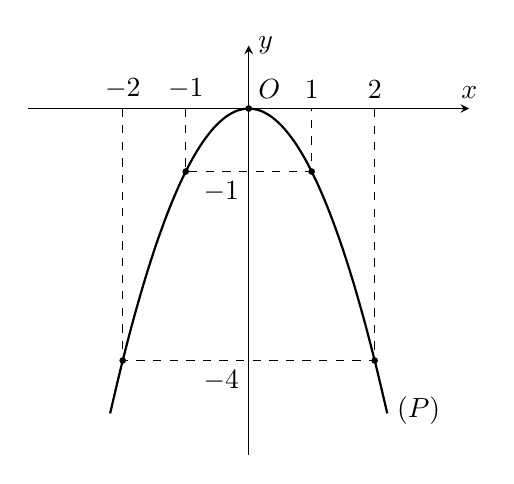
\begin{tikzpicture}[>=stealth, scale=0.8]
\draw[->] (-3.5,0) -- (3.5,0) node[above] {$x$};
\draw[->] (0,-5.5) -- (0,1) node[right] {$y$};
\fill (0,0) circle (1.5pt) node[above right] {$O$};
\draw[domain=-2.2:2.2, smooth, thick] plot (\x, {-\x*\x});
\draw[dashed] (-2,0) node[above]{$-2$} |- (0,-4) node[below left]{$-4$} -| (2,0) node[above]{$2$};
\draw[dashed] (-1,0) node[above]{$-1$} |- (0,-1) node[below left]{$-1$} -| (1,0) node[above]{$1$};
\fill (-2,-4) circle (1.5pt); \fill (2,-4) circle (1.5pt);
\fill (-1,-1) circle (1.5pt); \fill (1,-1) circle (1.5pt);
\node[right] at (2.2, -4.8) {$(P)$};
\end{tikzpicture}
\end{center}
\textbf{b)} Tìm tọa độ các điểm $M$ \hfill \textit{(0,5 điểm)} \par
Gọi tọa độ điểm $M$ là $(x_M; y_M)$. Vì $M \in (P)$ nên $y_M = -x_M^2$. \par
Theo đề bài, hiệu của hoành độ và tung độ bằng $2$, ta có phương trình:
$$ x_M - y_M = 2 $$
$$ \Leftrightarrow x_M - (-x_M^2) = 2 $$
$$ \Leftrightarrow x_M^2 + x_M - 2 = 0 $$
Vì $a + b + c = 1 + 1 + (-2) = 0$ nên phương trình có hai nghiệm:
$$ x_{M1} = 1; \quad x_{M2} = -2 $$
Với $x_M = 1 \Rightarrow y_M = -(1)^2 = -1$, ta được điểm $M_1(1; -1)$. \par
Với $x_M = -2 \Rightarrow y_M = -(-2)^2 = -4$, ta được điểm $M_2(-2; -4)$. \par
Vậy tọa độ các điểm $M$ cần tìm là $(1; -1)$ và $(-2; -4)$.
}
\end{bt}

\begin{bt}%[9D6H18-3]%[ma:3f40a071]
% nguon: Tuyển tập đề thi Tuyển sinh 10 TP.HCM
Cho parabol $(P): y = x^2$ và đường thẳng $(d): y = -2x + 3$.
\textbf{a)} Vẽ đồ thị $(P)$ trên hệ trục tọa độ. \par
\textbf{b)} Tìm tọa độ giao điểm của $(P)$ và $(d)$ bằng phép tính.
\loigiai{
\textbf{a)} Vẽ đồ thị $(P): y = x^2$ \hfill \textit{(1,0 điểm)} \par
Bảng giá trị:
\begin{center}
\begin{tabular}{|c|c|c|c|c|c|}
\hline
$x$ & $-2$ & $-1$ & $0$ & $1$ & $2$ \\
\hline
$y = x^2$ & $4$ & $1$ & $0$ & $1$ & $4$ \\
\hline
\end{tabular}
\end{center}
Đồ thị hàm số $(P)$ là một đường parabol đi qua gốc tọa độ $O$, nhận trục $Oy$ làm trục đối xứng và nằm phía trên trục hoành.
\begin{center}
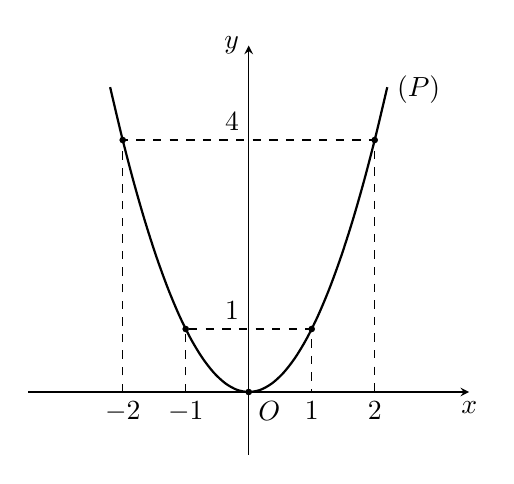
\begin{tikzpicture}[>=stealth, scale=0.8]
\draw[->] (-3.5,0) -- (3.5,0) node[below] {$x$};
\draw[->] (0,-1) -- (0,5.5) node[left] {$y$};
\fill (0,0) circle (1.5pt) node[below right] {$O$};
\draw[domain=-2.2:2.2, smooth, thick] plot (\x, {\x*\x});
\draw[dashed] (-2,0) node[below]{$-2$} |- (0,4) node[above left]{$4$} -| (2,0) node[below]{$2$};
\draw[dashed] (-1,0) node[below]{$-1$} |- (0,1) node[above left]{$1$} -| (1,0) node[below]{$1$};
\fill (-2,4) circle (1.5pt); \fill (2,4) circle (1.5pt);
\fill (-1,1) circle (1.5pt); \fill (1,1) circle (1.5pt);
\node[right] at (2.2, 4.8) {$(P)$};
\end{tikzpicture}
\end{center}
\textbf{b)} Tìm tọa độ giao điểm của $(P)$ và $(d)$ \hfill \textit{(0,5 điểm)} \par
Phương trình hoành độ giao điểm của $(P)$ và $(d)$ là:
$$ x^2 = -2x + 3 $$
$$ \Leftrightarrow x^2 + 2x - 3 = 0 $$
Vì $a + b + c = 1 + 2 + (-3) = 0$ nên phương trình có hai nghiệm:
$$ x_1 = 1; \quad x_2 = -3 $$
Với $x = 1 \Rightarrow y = (1)^2 = 1$. Ta được giao điểm thứ nhất là $(1; 1)$. \par
Với $x = -3 \Rightarrow y = (-3)^2 = 9$. Ta được giao điểm thứ hai là $(-3; 9)$. \par
Vậy tọa độ giao điểm của $(P)$ và $(d)$ là $(1; 1)$ và $(-3; 9)$.
}
\end{bt}

\begin{bt}%[9D6H18-2]%[ma:713c727b]
% nguon: Tuyển tập đề thi Tuyển sinh 10 TP.HCM
Cho parabol $(P): y = 2x^2$.
\textbf{a)} Vẽ đồ thị $(P)$ trên hệ trục tọa độ. \par
\textbf{b)} Tìm tọa độ các điểm $E$ thuộc $(P)$ sao cho tổng hoành độ và tung độ của điểm đó bằng $3$.
\loigiai{
\textbf{a)} Vẽ đồ thị $(P): y = 2x^2$ \hfill \textit{(1,0 điểm)} \par
Bảng giá trị:
\begin{center}
\begin{tabular}{|c|c|c|c|c|c|}
\hline
$x$ & $-2$ & $-1$ & $0$ & $1$ & $2$ \\
\hline
$y = 2x^2$ & $8$ & $2$ & $0$ & $2$ & $8$ \\
\hline
\end{tabular}
\end{center}
Đồ thị hàm số $(P)$ là một đường parabol đi qua gốc tọa độ $O$, nhận trục $Oy$ làm trục đối xứng và nằm phía trên trục hoành.
\begin{center}
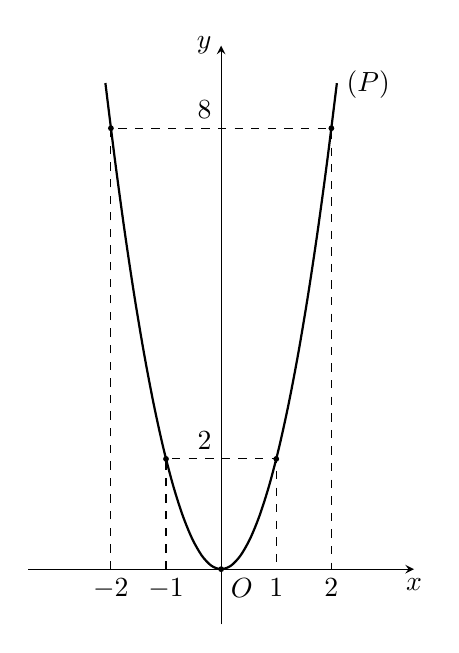
\begin{tikzpicture}[>=stealth, scale=0.7]
\draw[->] (-3.5,0) -- (3.5,0) node[below] {$x$};
\draw[->] (0,-1) -- (0,9.5) node[left] {$y$};
\fill (0,0) circle (1.5pt) node[below right] {$O$};
\draw[domain=-2.1:2.1, smooth, thick] plot (\x, {2*\x*\x});
\draw[dashed] (-2,0) node[below]{$-2$} |- (0,8) node[above left]{$8$} -| (2,0) node[below]{$2$};
\draw[dashed] (-1,0) node[below]{$-1$} |- (0,2) node[above left]{$2$} -| (1,0) node[below]{$1$};
\fill (-2,8) circle (1.5pt); \fill (2,8) circle (1.5pt);
\fill (-1,2) circle (1.5pt); \fill (1,2) circle (1.5pt);
\node[right] at (2.1, 8.8) {$(P)$};
\end{tikzpicture}
\end{center}
\textbf{b)} Tìm tọa độ các điểm $E$ \hfill \textit{(0,5 điểm)} \par
Gọi tọa độ điểm $E$ là $(x_E; y_E)$. Vì $E \in (P)$ nên $y_E = 2x_E^2$. \par
Theo đề bài, tổng hoành độ và tung độ bằng $3$, ta có phương trình:
$$ x_E + y_E = 3 $$
$$ \Leftrightarrow x_E + 2x_E^2 = 3 $$
$$ \Leftrightarrow 2x_E^2 + x_E - 3 = 0 $$
Vì $a + b + c = 2 + 1 + (-3) = 0$ nên phương trình có hai nghiệm:
$$ x_{E1} = 1; \quad x_{E2} = -\frac{3}{2} $$
Với $x_E = 1 \Rightarrow y_E = 2(1)^2 = 2$, ta được điểm $E_1(1; 2)$. \par
Với $x_E = -\frac{3}{2} \Rightarrow y_E = 2\left(-\frac{3}{2}\right)^2 = \frac{9}{2}$, ta được điểm $E_2\left(-\frac{3}{2}; \frac{9}{2}\right)$. \par
Vậy tọa độ các điểm $E$ cần tìm là $(1; 2)$ và $\left(-\frac{3}{2}; \frac{9}{2}\right)$.
}
\end{bt}

\begin{bt}%[9D6H18-3]%[ma:02d569b7]
% nguon: Tuyển tập đề thi Tuyển sinh 10 TP.HCM
Cho parabol $(P): y = 2x^2$ và đường thẳng $(d): y = x + 3$.
\textbf{a)} Vẽ đồ thị $(P)$ trên hệ trục tọa độ. \par
\textbf{b)} Tìm tọa độ giao điểm của $(P)$ và $(d)$ bằng phép tính.
\loigiai{
\textbf{a)} Vẽ đồ thị $(P): y = 2x^2$ \hfill \textit{(1,0 điểm)} \par
Bảng giá trị:
\begin{center}
\begin{tabular}{|c|c|c|c|c|c|}
\hline
$x$ & $-2$ & $-1$ & $0$ & $1$ & $2$ \\
\hline
$y = 2x^2$ & $8$ & $2$ & $0$ & $2$ & $8$ \\
\hline
\end{tabular}
\end{center}
Đồ thị hàm số $(P)$ là một đường parabol đi qua gốc tọa độ $O$, nhận trục $Oy$ làm trục đối xứng và nằm phía trên trục hoành.
\begin{center}
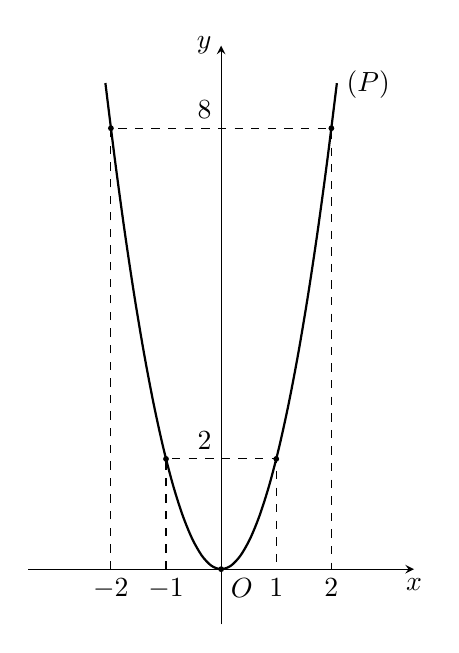
\begin{tikzpicture}[>=stealth, scale=0.7]
\draw[->] (-3.5,0) -- (3.5,0) node[below] {$x$};
\draw[->] (0,-1) -- (0,9.5) node[left] {$y$};
\fill (0,0) circle (1.5pt) node[below right] {$O$};
\draw[domain=-2.1:2.1, smooth, thick] plot (\x, {2*\x*\x});
\draw[dashed] (-2,0) node[below]{$-2$} |- (0,8) node[above left]{$8$} -| (2,0) node[below]{$2$};
\draw[dashed] (-1,0) node[below]{$-1$} |- (0,2) node[above left]{$2$} -| (1,0) node[below]{$1$};
\fill (-2,8) circle (1.5pt); \fill (2,8) circle (1.5pt);
\fill (-1,2) circle (1.5pt); \fill (1,2) circle (1.5pt);
\node[right] at (2.1, 8.8) {$(P)$};
\end{tikzpicture}
\end{center}
\textbf{b)} Tìm tọa độ giao điểm của $(P)$ và $(d)$ \hfill \textit{(0,5 điểm)} \par
Phương trình hoành độ giao điểm của $(P)$ và $(d)$ là:
$$ 2x^2 = x + 3 $$
$$ \Leftrightarrow 2x^2 - x - 3 = 0 $$
Vì $a - b + c = 2 - (-1) + (-3) = 0$ nên phương trình có hai nghiệm:
$$ x_1 = -1; \quad x_2 = \frac{3}{2} $$
Với $x = -1 \Rightarrow y = 2(-1)^2 = 2$. Ta được giao điểm thứ nhất là $(-1; 2)$. \par
Với $x = \frac{3}{2} \Rightarrow y = 2\left(\frac{3}{2}\right)^2 = \frac{9}{2}$. Ta được giao điểm thứ hai là $\left(\frac{3}{2}; \frac{9}{2}\right)$. \par
Vậy tọa độ giao điểm của $(P)$ và $(d)$ là $(-1; 2)$ và $\left(\frac{3}{2}; \frac{9}{2}\right)$.
}
\end{bt}

\begin{bt}%[9D6H18-2]%[ma:d4ba117e]
% nguon: Tuyển tập đề thi Tuyển sinh 10 TP.HCM
Cho parabol $(P): y = \frac{1}{2}x^2$.
\textbf{a)} Vẽ đồ thị $(P)$ trên mặt phẳng tọa độ. \par
\textbf{b)} Bằng phép tính, hãy kiểm tra xem các điểm $A(4; 8)$ và $B(-2; 3)$ có thuộc đồ thị $(P)$ hay không?
\loigiai{
\textbf{a)} Vẽ đồ thị $(P)$ \hfill \textit{(1,0 điểm)}\par
Bảng giá trị:
\begin{center}
\begin{tabular}{|c|c|c|c|c|c|}
\hline
$x$ & $-4$ & $-2$ & $0$ & $2$ & $4$ \\
\hline
$y = \frac{1}{2}x^2$ & $8$ & $2$ & $0$ & $2$ & $8$ \\
\hline
\end{tabular}
\end{center}
Đồ thị hàm số $(P)$ là một đường parabol đi qua gốc tọa độ $O$, nhận trục $Oy$ làm trục đối xứng và nằm phía trên trục hoành.
\begin{center}
\begin{tikzpicture}[>=stealth, scale=0.7]
\draw[->] (-5,0) -- (5,0) node[below] {$x$};
\draw[->] (0,-1) -- (0,9) node[left] {$y$};
\fill (0,0) circle (1.5pt) node[below right] {$O$};
\draw[domain=-4.2:4.2, smooth, thick] plot (\x, {0.5*\x*\x});
\draw[dashed] (-4,0) node[below]{$-4$} |- (0,8) node[above left]{$8$} -| (4,0) node[below]{$4$};
\draw[dashed] (-2,0) node[below]{$-2$} |- (0,2) node[above left]{$2$} -| (2,0) node[below]{$2$};
\fill (-4,8) circle (1.5pt); \fill (4,8) circle (1.5pt);
\fill (-2,2) circle (1.5pt); \fill (2,2) circle (1.5pt);
\node[right] at (4.2, 8.8) {$(P)$};
\end{tikzpicture}
\end{center}
\textbf{b)} Kiểm tra các điểm $A, B$ \hfill \textit{(0,5 điểm)}\par
Xét điểm $A(4; 8)$: Thay $x = 4$ vào hàm số của $(P)$, ta được:
$$ y = \frac{1}{2} \cdot 4^2 = \frac{1}{2} \cdot 16 = 8 $$
Giá trị này bằng với tung độ của điểm $A$, nên điểm $A(4; 8)$ thuộc $(P)$.\par
Xét điểm $B(-2; 3)$: Thay $x = -2$ vào hàm số của $(P)$, ta được:
$$ y = \frac{1}{2} \cdot (-2)^2 = \frac{1}{2} \cdot 4 = 2 $$
Giá trị này khác tung độ của điểm $B$ ($2 \neq 3$), nên điểm $B(-2; 3)$ không thuộc $(P)$.
}
\end{bt}

\begin{bt}%[9D6H18-2]%[ma:351f32e2]
% nguon: Tuyển tập đề thi Tuyển sinh 10 TP.HCM
Cho hàm số $y = x^2$ có đồ thị là parabol $(P)$.
\textbf{a)} Vẽ đồ thị $(P)$ trên hệ trục tọa độ. \par
\textbf{b)} Tìm tọa độ hai điểm $A, B$ thuộc $(P)$ (khác gốc tọa độ $O$) sao cho $A, B$ đối xứng nhau qua trục $Oy$ và tam giác $OAB$ vuông cân tại $O$.
\loigiai{
\textbf{a)} Vẽ đồ thị $(P)$ \hfill \textit{(1,0 điểm)}\par
Bảng giá trị:
\begin{center}
\begin{tabular}{|c|c|c|c|c|c|}
\hline
$x$ & $-2$ & $-1$ & $0$ & $1$ & $2$ \\
\hline
$y = x^2$ & $4$ & $1$ & $0$ & $1$ & $4$ \\
\hline
\end{tabular}
\end{center}
Đồ thị hàm số $(P)$ là đường parabol đi qua gốc tọa độ $O$, nhận trục $Oy$ làm trục đối xứng và nằm phía trên trục hoành.
\begin{center}
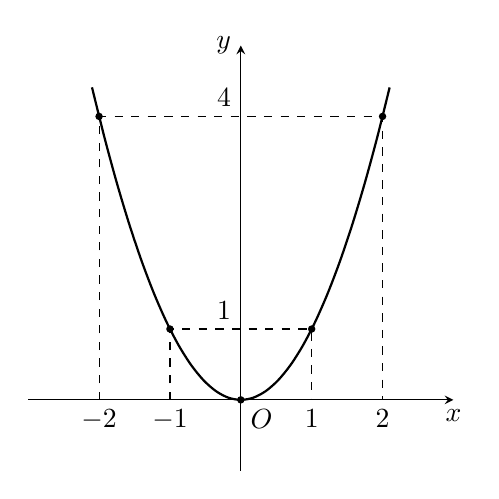
\begin{tikzpicture}[>=stealth, scale=0.9]
\draw[->] (-3,0) -- (3,0) node[below] {$x$};
\draw[->] (0,-1) -- (0,5) node[left] {$y$};
\fill (0,0) circle (1.5pt) node[below right] {$O$};
\draw[domain=-2.1:2.1, smooth, thick] plot (\x, {\x*\x});
\draw[dashed] (-2,0) node[below]{$-2$} |- (0,4) node[above left]{$4$} -| (2,0) node[below]{$2$};
\draw[dashed] (-1,0) node[below]{$-1$} |- (0,1) node[above left]{$1$} -| (1,0) node[below]{$1$};
\fill (-2,4) circle (1.5pt); \fill (2,4) circle (1.5pt);
\fill (-1,1) circle (1.5pt); \fill (1,1) circle (1.5pt);
\end{tikzpicture}
\end{center}
\textbf{b)} Tìm tọa độ hai điểm $A, B$ \hfill \textit{(0,5 điểm)}\par
Vì $A, B$ thuộc $(P)$ và đối xứng nhau qua trục $Oy$ nên ta gọi tọa độ điểm $B$ là $(x_0; x_0^2)$ với $x_0 > 0$. Khi đó tọa độ điểm $A$ là $(-x_0; x_0^2)$.\par
Độ dài đoạn thẳng $AB = x_0 - (-x_0) = 2x_0$.\par
Gọi $H$ là giao điểm của $AB$ và trục $Oy$, ta có $H(0; x_0^2)$. Suy ra $OH = x_0^2$.\par
Vì tam giác $OAB$ cân tại $O$ (do tính đối xứng) và vuông tại $O$, nên đường cao $OH$ đồng thời là đường trung tuyến ứng với cạnh huyền $AB$.
Do đó: $OH = \frac{1}{2}AB \Leftrightarrow x_0^2 = \frac{1}{2}(2x_0) \Leftrightarrow x_0^2 = x_0$.\par
Vì $x_0 > 0$ nên chia hai vế cho $x_0$, ta được $x_0 = 1$.\par
Với $x_0 = 1$, ta có $y_0 = 1^2 = 1$.\par
Vậy tọa độ hai điểm cần tìm là $A(-1; 1)$ và $B(1; 1)$.
}
\end{bt}

\begin{bt}%[9D6H18-2]%[ma:74517e8e]
% nguon: Tuyển tập đề thi Tuyển sinh 10 TP.HCM
Cho parabol $(P): y = -\frac{1}{4}x^2$.
\textbf{a)} Vẽ đồ thị $(P)$ trên mặt phẳng tọa độ $Oxy$. \par
\textbf{b)} Một vòm cầu có hình dạng parabol. Khi gắn hệ trục tọa độ sao cho đỉnh vòm cầu trùng với gốc tọa độ $O$ và vòm cầu nằm phía dưới trục hoành, người ta đo được bề rộng mặt cầu ở chân vòm là $8\text{ m}$ và chiều cao từ đỉnh vòm xuống chân vòm là $4\text{ m}$. Hỏi hình dạng của vòm cầu có khớp với đồ thị $(P)$ hay không? Vì sao?
\loigiai{
\textbf{a)} Vẽ đồ thị $(P)$ \hfill \textit{(1,0 điểm)}\par
Bảng giá trị:
\begin{center}
\begin{tabular}{|c|c|c|c|c|c|}
\hline
$x$ & $-4$ & $-2$ & $0$ & $2$ & $4$ \\
\hline
$y = -\frac{1}{4}x^2$ & $-4$ & $-1$ & $0$ & $-1$ & $-4$ \\
\hline
\end{tabular}
\end{center}
Đồ thị hàm số $(P)$ là đường parabol đi qua gốc tọa độ $O$, nhận trục $Oy$ làm trục đối xứng và nằm phía dưới trục hoành.
\begin{center}
\begin{tikzpicture}[>=stealth, scale=0.8]
\draw[->] (-5,0) -- (5,0) node[above] {$x$};
\draw[->] (0,-5) -- (0,1) node[right] {$y$};
\fill (0,0) circle (1.5pt) node[above right] {$O$};
\draw[domain=-4.2:4.2, smooth, thick] plot (\x, {-0.25*\x*\x});
\draw[dashed] (-4,0) node[above]{$-4$} |- (0,-4) node[below left]{$-4$} -| (4,0) node[above]{$4$};
\draw[dashed] (-2,0) node[above]{$-2$} |- (0,-1) node[below left]{$-1$} -| (2,0) node[above]{$2$};
\fill (-4,-4) circle (1.5pt); \fill (4,-4) circle (1.5pt);
\fill (-2,-1) circle (1.5pt); \fill (2,-1) circle (1.5pt);
\end{tikzpicture}
\end{center}
\textbf{b)} Kiểm tra sự khớp nhau của vòm cầu \hfill \textit{(0,5 điểm)}\par
Theo đề bài, bề rộng ở chân vòm là $8\text{ m}$, do tính đối xứng, mỗi bên gốc tọa độ rộng $4\text{ m}$, suy ra hoành độ chân vòm là $x = 4$ và $x = -4$.\par
Chiều cao từ đỉnh vòm (gốc $O$) xuống chân vòm là $4\text{ m}$ và vòm cầu nằm dưới trục hoành, nên tung độ của chân vòm là $y = -4$.\par
Như vậy, hai điểm ở chân vòm có tọa độ là $(4; -4)$ và $(-4; -4)$.\par
Ta kiểm tra xem điểm $(4; -4)$ có thuộc đồ thị $(P): y = -\frac{1}{4}x^2$ hay không:
Thay $x = 4$ vào phương trình $(P)$, ta có: $y = -\frac{1}{4} \cdot 4^2 = -\frac{1}{4} \cdot 16 = -4$ (đúng bằng tung độ của điểm).\par
Do parabol có tính đối xứng nên điểm $(-4; -4)$ cũng thuộc $(P)$.\par
Vậy hình dạng vòm cầu hoàn toàn khớp với đồ thị của $(P)$.
}
\end{bt}

\begin{bt}%[9D6H18-2]%[ma:2ccdfb7a]
% nguon: Tuyển tập đề thi Tuyển sinh 10 TP.HCM
Cho hàm số $y = -x^2$ có đồ thị là $(P)$.
\textbf{a)} Vẽ đồ thị $(P)$ trên hệ trục tọa độ. \par
\textbf{b)} Quỹ đạo của một tia nước từ một đài phun nước được mô phỏng bởi parabol $(P)$ (đơn vị trên các trục tính bằng mét). Một tia laser màu đỏ được chiếu ngang qua đài phun nước tại độ cao $y = -9$ (tức là cách đỉnh tia nước $9\text{ m}$ về phía dưới). Tính khoảng cách theo phương ngang giữa hai điểm mà tia nước cắt tia laser.
\loigiai{
\textbf{a)} Vẽ đồ thị $(P)$ \hfill \textit{(1,0 điểm)}\par
Bảng giá trị:
\begin{center}
\begin{tabular}{|c|c|c|c|c|c|}
\hline
$x$ & $-2$ & $-1$ & $0$ & $1$ & $2$ \\
\hline
$y = -x^2$ & $-4$ & $-1$ & $0$ & $-1$ & $-4$ \\
\hline
\end{tabular}
\end{center}
Đồ thị hàm số $(P)$ là đường parabol đi qua gốc tọa độ $O$, nhận trục $Oy$ làm trục đối xứng và nằm phía dưới trục hoành.
\begin{center}
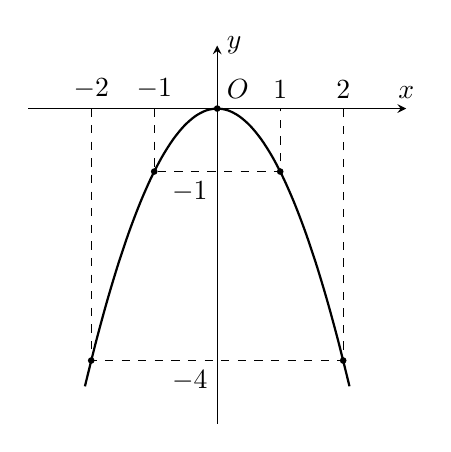
\begin{tikzpicture}[>=stealth, scale=0.8]
\draw[->] (-3,0) -- (3,0) node[above] {$x$};
\draw[->] (0,-5) -- (0,1) node[right] {$y$};
\fill (0,0) circle (1.5pt) node[above right] {$O$};
\draw[domain=-2.1:2.1, smooth, thick] plot (\x, {-\x*\x});
\draw[dashed] (-2,0) node[above]{$-2$} |- (0,-4) node[below left]{$-4$} -| (2,0) node[above]{$2$};
\draw[dashed] (-1,0) node[above]{$-1$} |- (0,-1) node[below left]{$-1$} -| (1,0) node[above]{$1$};
\fill (-2,-4) circle (1.5pt); \fill (2,-4) circle (1.5pt);
\fill (-1,-1) circle (1.5pt); \fill (1,-1) circle (1.5pt);
\end{tikzpicture}
\end{center}
\textbf{b)} Tính khoảng cách \hfill \textit{(0,5 điểm)}\par
Giao điểm của tia nước và tia laser là các điểm thuộc đồ thị $(P)$ có tung độ $y = -9$.\par
Thay $y = -9$ vào phương trình $(P)$, ta được:
$$ -x^2 = -9 \Leftrightarrow x^2 = 9 \Leftrightarrow x = 3 \text{ hoặc } x = -3 $$
Hai điểm cắt nhau có tọa độ lần lượt là $A(-3; -9)$ và $B(3; -9)$.\par
Khoảng cách theo phương ngang giữa hai điểm này là khoảng cách giữa hai hoành độ:
$$ AB = |3 - (-3)| = 6\text{ (m)} $$
Vậy khoảng cách theo phương ngang cần tìm là $6\text{ m}$.
}
\end{bt}

\begin{bt}%[9D6H18-3]%[ma:2d79bb6c]
% nguon: Tuyển tập đề thi Tuyển sinh 10 TP.HCM
Cho parabol $(P): y = \frac{1}{4}x^2$.
\textbf{a)} Vẽ đồ thị $(P)$ trên mặt phẳng tọa độ. \par
\textbf{b)} Gọi $A$ và $B$ là hai điểm thuộc $(P)$ có hoành độ lần lượt là $-2$ và $4$. Tính diện tích tam giác $OAB$.
\loigiai{
\textbf{a)} Vẽ đồ thị $(P)$ \hfill \textit{(1,0 điểm)}\par
Bảng giá trị:
\begin{center}
\begin{tabular}{|c|c|c|c|c|c|}
\hline
$x$ & $-4$ & $-2$ & $0$ & $2$ & $4$ \\
\hline
$y = \frac{1}{4}x^2$ & $4$ & $1$ & $0$ & $1$ & $4$ \\
\hline
\end{tabular}
\end{center}
Đồ thị hàm số $(P)$ là đường parabol đi qua gốc tọa độ $O$, nhận trục $Oy$ làm trục đối xứng và nằm phía trên trục hoành.
\begin{center}
\begin{tikzpicture}[>=stealth, scale=0.8]
\draw[->] (-5,0) -- (5,0) node[below] {$x$};
\draw[->] (0,-1) -- (0,5) node[left] {$y$};
\fill (0,0) circle (1.5pt) node[below right] {$O$};
\draw[domain=-4.2:4.2, smooth, thick] plot (\x, {0.25*\x*\x});
\draw[dashed] (-4,0) node[below]{$-4$} |- (0,4) node[above left]{$4$} -| (4,0) node[below]{$4$};
\draw[dashed] (-2,0) node[below]{$-2$} |- (0,1) node[above left]{$1$} -| (2,0) node[below]{$2$};
\fill (-4,4) circle (1.5pt); \fill (4,4) circle (1.5pt);
\fill (-2,1) circle (1.5pt); \fill (2,1) circle (1.5pt);
\end{tikzpicture}
\end{center}
\textbf{b)} Tính diện tích tam giác $OAB$ \hfill \textit{(0,5 điểm)}\par
Với $x_A = -2 \Rightarrow y_A = \frac{1}{4}(-2)^2 = 1$. Ta có $A(-2; 1)$.\par
Với $x_B = 4 \Rightarrow y_B = \frac{1}{4}(4)^2 = 4$. Ta có $B(4; 4)$.\par
Gọi phương trình đường thẳng $AB$ là $y = ax + b$.
Thay tọa độ $A, B$ vào, ta có hệ:
$$ \heva{&-2a + b = 1 \\ &4a + b = 4} \Leftrightarrow \heva{&6a = 3 \\ &b = 1 + 2a} \Leftrightarrow \heva{&a = \frac{1}{2} \\ &b = 2} $$
Đường thẳng $AB$ có phương trình $y = \frac{1}{2}x + 2$. Gọi $C$ là giao điểm của $AB$ với trục $Oy$, ta có $C(0; 2) \Rightarrow OC = 2$.\par
Diện tích tam giác $OAB$ được chia thành hai tam giác vuông $OAC$ và $OBC$ chung cạnh đáy $OC$:
$$ S_{OAB} = S_{OAC} + S_{OBC} = \frac{1}{2} \cdot OC \cdot |x_A| + \frac{1}{2} \cdot OC \cdot |x_B| $$
$$ S_{OAB} = \frac{1}{2} \cdot 2 \cdot |-2| + \frac{1}{2} \cdot 2 \cdot |4| = 2 + 4 = 6 \text{ (đvdt).} $$
}
\end{bt}

\begin{bt}%[9D6H18-2]%[ma:c6a45f7f]
% nguon: Tuyển tập đề thi Tuyển sinh 10 TP.HCM
Cho hàm số $y = 2x^2$ có đồ thị là $(P)$.
\textbf{a)} Vẽ $(P)$ trên hệ trục tọa độ. \par
\textbf{b)} Bằng phép tính, hãy xác định xem các điểm $E(3; 18)$ và $F(-\sqrt{2}; 4)$ có nằm trên đồ thị $(P)$ hay không?
\loigiai{
\textbf{a)} Vẽ đồ thị $(P)$ \hfill \textit{(1,0 điểm)}\par
Bảng giá trị:
\begin{center}
\begin{tabular}{|c|c|c|c|c|c|}
\hline
$x$ & $-2$ & $-1$ & $0$ & $1$ & $2$ \\
\hline
$y = 2x^2$ & $8$ & $2$ & $0$ & $2$ & $8$ \\
\hline
\end{tabular}
\end{center}
Đồ thị hàm số $(P)$ là đường parabol đi qua gốc tọa độ $O$, nhận trục $Oy$ làm trục đối xứng và nằm phía trên trục hoành.
\begin{center}
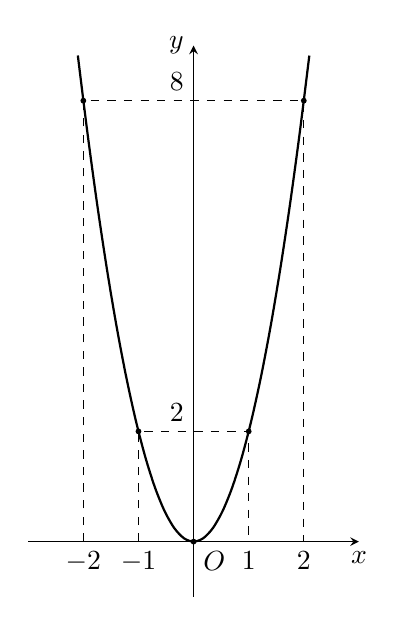
\begin{tikzpicture}[>=stealth, scale=0.7]
\draw[->] (-3,0) -- (3,0) node[below] {$x$};
\draw[->] (0,-1) -- (0,9) node[left] {$y$};
\fill (0,0) circle (1.5pt) node[below right] {$O$};
\draw[domain=-2.1:2.1, smooth, thick] plot (\x, {2*\x*\x});
\draw[dashed] (-2,0) node[below]{$-2$} |- (0,8) node[above left]{$8$} -| (2,0) node[below]{$2$};
\draw[dashed] (-1,0) node[below]{$-1$} |- (0,2) node[above left]{$2$} -| (1,0) node[below]{$1$};
\fill (-2,8) circle (1.5pt); \fill (2,8) circle (1.5pt);
\fill (-1,2) circle (1.5pt); \fill (1,2) circle (1.5pt);
\end{tikzpicture}
\end{center}
\textbf{b)} Xác định các điểm $E, F$ \hfill \textit{(0,5 điểm)}\par
Xét điểm $E(3; 18)$: Thay hoành độ $x = 3$ vào hàm số của $(P)$, ta được:
$$ y = 2 \cdot 3^2 = 2 \cdot 9 = 18 $$
Đúng bằng tung độ của điểm $E$, nên điểm $E(3; 18)$ nằm trên $(P)$.\par
Xét điểm $F(-\sqrt{2}; 4)$: Thay hoành độ $x = -\sqrt{2}$ vào hàm số của $(P)$, ta được:
$$ y = 2 \cdot (-\sqrt{2})^2 = 2 \cdot 2 = 4 $$
Đúng bằng tung độ của điểm $F$, nên điểm $F(-\sqrt{2}; 4)$ cũng nằm trên $(P)$.\par
Vậy cả hai điểm $E$ và $F$ đều nằm trên đồ thị $(P)$.
}
\end{bt}

\begin{bt}%[9D6H18-3]%[ma:05be1f49]
% nguon: Tuyển tập đề thi Tuyển sinh 10 TP.HCM
Cho parabol $(P): y = -\frac{1}{2}x^2$.
\textbf{a)} Vẽ đồ thị $(P)$ trên hệ trục tọa độ. \par
\textbf{b)} Một cổng vòm có dạng parabol $(P)$ với đơn vị đo trên các trục là mét. Biết rằng mặt đường đi ngang qua vòm cầu ứng với đường thẳng $y = -2$. Tính bề rộng của mặt đường đi dưới cổng vòm đó.
\loigiai{
\textbf{a)} Vẽ đồ thị $(P)$ \hfill \textit{(1,0 điểm)}\par
Bảng giá trị:
\begin{center}
\begin{tabular}{|c|c|c|c|c|c|}
\hline
$x$ & $-4$ & $-2$ & $0$ & $2$ & $4$ \\
\hline
$y = -\frac{1}{2}x^2$ & $-8$ & $-2$ & $0$ & $-2$ & $-8$ \\
\hline
\end{tabular}
\end{center}
Đồ thị hàm số $(P)$ là đường parabol đi qua gốc tọa độ $O$, nhận trục $Oy$ làm trục đối xứng và nằm phía dưới trục hoành.
\begin{center}
\begin{tikzpicture}[>=stealth, scale=0.7]
\draw[->] (-5,0) -- (5,0) node[above] {$x$};
\draw[->] (0,-9) -- (0,1) node[right] {$y$};
\fill (0,0) circle (1.5pt) node[above right] {$O$};
\draw[domain=-4.2:4.2, smooth, thick] plot (\x, {-0.5*\x*\x});
\draw[dashed] (-4,0) node[above]{$-4$} |- (0,-8) node[below left]{$-8$} -| (4,0) node[above]{$4$};
\draw[dashed] (-2,0) node[above]{$-2$} |- (0,-2) node[below left]{$-2$} -| (2,0) node[above]{$2$};
\fill (-4,-8) circle (1.5pt); \fill (4,-8) circle (1.5pt);
\fill (-2,-2) circle (1.5pt); \fill (2,-2) circle (1.5pt);
\end{tikzpicture}
\end{center}
\textbf{b)} Tính bề rộng mặt đường \hfill \textit{(0,5 điểm)}\par
Mặt đường tương ứng với các điểm trên $(P)$ có tung độ $y = -2$. Ta xét phương trình:
$$ -\frac{1}{2}x^2 = -2 \Leftrightarrow x^2 = 4 \Leftrightarrow \heva{&x = 2 \\ &x = -2} $$
Do đó, cổng vòm chạm mặt đường tại hai điểm có tọa độ $(2; -2)$ và $(-2; -2)$.\par
Bề rộng của mặt đường đi dưới cổng vòm chính là khoảng cách giữa hai hoành độ này:
$$ \text{Bề rộng} = 2 - (-2) = 4 \text{ (m)} $$
Vậy bề rộng của mặt đường đi dưới cổng vòm là $4\text{ m}$.
}
\end{bt}

\begin{bt}%[9D6H18-3]%[ma:0e41f170]
% nguon: Tuyển tập đề thi Tuyển sinh 10 TP.HCM
Cho hàm số $y = -2x^2$ có đồ thị là $(P)$.
\textbf{a)} Vẽ $(P)$ trên mặt phẳng tọa độ $Oxy$. \par
\textbf{b)} Đường thẳng $d: y = -8$ cắt đồ thị $(P)$ tại hai điểm phân biệt $M, N$. Tính chu vi tam giác $OMN$.
\loigiai{
\textbf{a)} Vẽ đồ thị $(P)$ \hfill \textit{(1,0 điểm)}\par
Bảng giá trị:
\begin{center}
\begin{tabular}{|c|c|c|c|c|c|}
\hline
$x$ & $-2$ & $-1$ & $0$ & $1$ & $2$ \\
\hline
$y = -2x^2$ & $-8$ & $-2$ & $0$ & $-2$ & $-8$ \\
\hline
\end{tabular}
\end{center}
Đồ thị hàm số $(P)$ là đường parabol đi qua gốc tọa độ $O$, nhận trục $Oy$ làm trục đối xứng và nằm phía dưới trục hoành.
\begin{center}
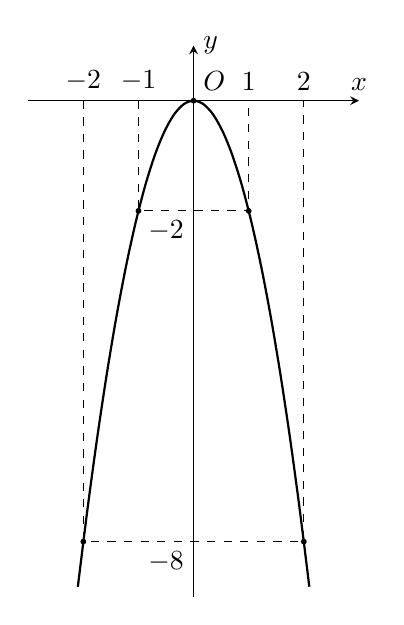
\begin{tikzpicture}[>=stealth, scale=0.7]
\draw[->] (-3,0) -- (3,0) node[above] {$x$};
\draw[->] (0,-9) -- (0,1) node[right] {$y$};
\fill (0,0) circle (1.5pt) node[above right] {$O$};
\draw[domain=-2.1:2.1, smooth, thick] plot (\x, {-2*\x*\x});
\draw[dashed] (-2,0) node[above]{$-2$} |- (0,-8) node[below left]{$-8$} -| (2,0) node[above]{$2$};
\draw[dashed] (-1,0) node[above]{$-1$} |- (0,-2) node[below left]{$-2$} -| (1,0) node[above]{$1$};
\fill (-2,-8) circle (1.5pt); \fill (2,-8) circle (1.5pt);
\fill (-1,-2) circle (1.5pt); \fill (1,-2) circle (1.5pt);
\end{tikzpicture}
\end{center}
\textbf{b)} Tính chu vi tam giác $OMN$ \hfill \textit{(0,5 điểm)}\par
Phương trình hoành độ giao điểm của $(P)$ và $d$:
$$ -2x^2 = -8 \Leftrightarrow x^2 = 4 \Leftrightarrow x = \pm 2 $$
Ta được tọa độ hai giao điểm là $M(-2; -8)$ và $N(2; -8)$.\par
Độ dài cạnh $MN = 2 - (-2) = 4$.\par
Áp dụng định lý Pythagore để tính $OM$ và $ON$ (với $OM = ON$ do tính đối xứng):
$$ OM = \sqrt{(-2)^2 + (-8)^2} = \sqrt{4 + 64} = \sqrt{68} = 2\sqrt{17} $$
Do đó $ON = 2\sqrt{17}$.\par
Chu vi tam giác $OMN$ là:
$$ P = OM + ON + MN = 2\sqrt{17} + 2\sqrt{17} + 4 = 4 + 4\sqrt{17} \text{ (đvđd).} $$
}
\end{bt}

\begin{bt}%[9D6H18-2]%[ma:6cfca531]
% nguon: Tuyển tập đề thi Tuyển sinh 10 TP.HCM
Cho parabol $(P): y = \frac{x^2}{2}$.
\textbf{a)} Vẽ đồ thị $(P)$ trên hệ trục tọa độ. \par
\textbf{b)} Tìm tham số $m$ để điểm $K(2m; 8)$ thuộc đồ thị $(P)$.
\loigiai{
\textbf{a)} Vẽ đồ thị $(P)$ \hfill \textit{(1,0 điểm)}\par
Bảng giá trị:
\begin{center}
\begin{tabular}{|c|c|c|c|c|c|}
\hline
$x$ & $-4$ & $-2$ & $0$ & $2$ & $4$ \\
\hline
$y = \frac{x^2}{2}$ & $8$ & $2$ & $0$ & $2$ & $8$ \\
\hline
\end{tabular}
\end{center}
Đồ thị hàm số $(P)$ là đường parabol đi qua gốc tọa độ $O$, nhận trục $Oy$ làm trục đối xứng và nằm phía trên trục hoành.
\begin{center}
\begin{tikzpicture}[>=stealth, scale=0.7]
\draw[->] (-5,0) -- (5,0) node[below] {$x$};
\draw[->] (0,-1) -- (0,9) node[left] {$y$};
\fill (0,0) circle (1.5pt) node[below right] {$O$};
\draw[domain=-4.2:4.2, smooth, thick] plot (\x, {0.5*\x*\x});
\draw[dashed] (-4,0) node[below]{$-4$} |- (0,8) node[above left]{$8$} -| (4,0) node[below]{$4$};
\draw[dashed] (-2,0) node[below]{$-2$} |- (0,2) node[above left]{$2$} -| (2,0) node[below]{$2$};
\fill (-4,8) circle (1.5pt); \fill (4,8) circle (1.5pt);
\fill (-2,2) circle (1.5pt); \fill (2,2) circle (1.5pt);
\end{tikzpicture}
\end{center}
\textbf{b)} Tìm tham số $m$ \hfill \textit{(0,5 điểm)}\par
Vì điểm $K(2m; 8)$ thuộc đồ thị $(P): y = \frac{x^2}{2}$, ta thay $x = 2m$ và $y = 8$ vào hàm số, ta được:
$$ 8 = \frac{(2m)^2}{2} $$
$$ \Leftrightarrow 8 = \frac{4m^2}{2} $$
$$ \Leftrightarrow 8 = 2m^2 $$
$$ \Leftrightarrow m^2 = 4 $$
$$ \Leftrightarrow m = 2 \text{ hoặc } m = -2 $$
Vậy các giá trị của tham số $m$ cần tìm là $m = 2$ hoặc $m = -2$.
}
\end{bt}

\begin{bt}%[9D6H18-2]%[ma:cd8cc7a4]
% nguon: Tuyển tập đề thi Tuyển sinh 10 TP.HCM
Cho hàm số $y = x^2$ có đồ thị $(P)$.
\textbf{a)} Vẽ đồ thị $(P)$ trên hệ trục tọa độ. \par
\textbf{b)} Mặt cắt mặt trước của một chảo ăng-ten vệ tinh có hình dạng parabol $(P)$ (đơn vị trên các trục tọa độ tính bằng đê-xi-mét). Người ta đo được chiều sâu của chảo (tính từ mặt đáy ở đỉnh $O$ lên đến miệng chảo) là $4\text{ dm}$. Hỏi đường kính miệng chảo ăng-ten đó bằng bao nhiêu?
\loigiai{
\textbf{a)} Vẽ đồ thị $(P)$ \hfill \textit{(1,0 điểm)}\par
Bảng giá trị:
\begin{center}
\begin{tabular}{|c|c|c|c|c|c|}
\hline
$x$ & $-2$ & $-1$ & $0$ & $1$ & $2$ \\
\hline
$y = x^2$ & $4$ & $1$ & $0$ & $1$ & $4$ \\
\hline
\end{tabular}
\end{center}
Đồ thị hàm số $(P)$ là đường parabol đi qua gốc tọa độ $O$, nhận trục $Oy$ làm trục đối xứng và nằm phía trên trục hoành.
\begin{center}
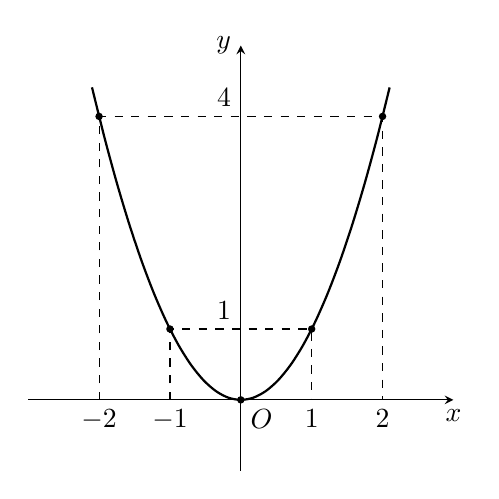
\begin{tikzpicture}[>=stealth, scale=0.9]
\draw[->] (-3,0) -- (3,0) node[below] {$x$};
\draw[->] (0,-1) -- (0,5) node[left] {$y$};
\fill (0,0) circle (1.5pt) node[below right] {$O$};
\draw[domain=-2.1:2.1, smooth, thick] plot (\x, {\x*\x});
\draw[dashed] (-2,0) node[below]{$-2$} |- (0,4) node[above left]{$4$} -| (2,0) node[below]{$2$};
\draw[dashed] (-1,0) node[below]{$-1$} |- (0,1) node[above left]{$1$} -| (1,0) node[below]{$1$};
\fill (-2,4) circle (1.5pt); \fill (2,4) circle (1.5pt);
\fill (-1,1) circle (1.5pt); \fill (1,1) circle (1.5pt);
\end{tikzpicture}
\end{center}
\textbf{b)} Tính đường kính miệng chảo \hfill \textit{(0,5 điểm)}\par
Chiều sâu của chảo là khoảng cách từ đỉnh đến miệng chảo, tức là tương ứng với tung độ $y = 4$.\par
Miệng chảo ứng với các điểm trên $(P)$ có tung độ $y = 4$. Thay vào phương trình hàm số, ta có:
$$ x^2 = 4 \Leftrightarrow x = 2 \text{ hoặc } x = -2 $$
Hai điểm ở mép miệng chảo có tọa độ là $(2; 4)$ và $(-2; 4)$.\par
Đường kính miệng chảo chính là khoảng cách giữa hai hoành độ này:
$$ d = 2 - (-2) = 4 \text{ (dm)} $$
Vậy đường kính miệng chảo ăng-ten đó là $4\text{ dm}$.
}
\end{bt}

\begin{bt}%[9D6H20-2]%[ma:dc26679d]
% nguon: Tuyển tập đề thi Tuyển sinh 10 TP.HCM
Cho phương trình: $2x^2 - x - 5 = 0$.
\textbf{a)} Chứng tỏ phương trình trên có hai nghiệm phân biệt $x_1, x_2$. \par
\textbf{b)} Không giải phương trình, hãy tính giá trị của biểu thức: $A = x_1^2 + x_2^2 - x_1 - x_2$.
\loigiai{
\textbf{a)} Chứng tỏ phương trình có hai nghiệm phân biệt \hfill \textit{(0,25 điểm)} \par
Phương trình $2x^2 - x - 5 = 0$ có hệ số $a = 2$, $c = -5$.
Ta có: $a \cdot c = 2 \cdot (-5) = -10 < 0$.
Do đó, phương trình luôn có hai nghiệm phân biệt $x_1, x_2$. \par
\textbf{b)} Tính giá trị của biểu thức $A$ \hfill \textit{(0,75 điểm)} \par
Theo định lí Viète, ta có:
$\heva{&S = x_1 + x_2 = \frac{1}{2} \\ &P = x_1 x_2 = -\frac{5}{2}}$ \par
Biến đổi biểu thức $A$:
$A = (x_1^2 + x_2^2) - (x_1 + x_2)$
$A = (x_1 + x_2)^2 - 2x_1 x_2 - (x_1 + x_2)$ \par
Thay các giá trị $S$ và $P$ vào biểu thức:
$A = \left(\frac{1}{2}\right)^2 - 2\left(-\frac{5}{2}\right) - \frac{1}{2}$
$A = \frac{1}{4} + 5 - \frac{1}{2} = \frac{1}{4} + \frac{20}{4} - \frac{2}{4} = \frac{19}{4}$. \par
Vậy $A = \frac{19}{4}$.
}
\end{bt}

\begin{bt}%[9D6H20-2]%[ma:c72a9adb]
% nguon: Tuyển tập đề thi Tuyển sinh 10 TP.HCM
Cho phương trình: $3x^2 + 4x - 2 = 0$.
\textbf{a)} Chứng minh phương trình luôn có hai nghiệm phân biệt $x_1, x_2$. \par
\textbf{b)} Không giải phương trình, hãy tính giá trị của biểu thức: $B = \frac{x_1}{x_2 + 1} + \frac{x_2}{x_1 + 1}$.
\loigiai{
\textbf{a)} Chứng minh phương trình có hai nghiệm phân biệt \hfill \textit{(0,25 điểm)} \par
Phương trình $3x^2 + 4x - 2 = 0$ có $a = 3$, $c = -2$.
Ta thấy $a \cdot c = 3 \cdot (-2) = -6 < 0$.
Suy ra phương trình luôn có hai nghiệm phân biệt $x_1, x_2$. \par
\textbf{b)} Tính giá trị của biểu thức $B$ \hfill \textit{(0,75 điểm)} \par
Theo định lí Viète, ta có:
$x_1 + x_2 = -\frac{4}{3}$ và $x_1 x_2 = -\frac{2}{3}$. \par
Quy đồng mẫu thức biểu thức $B$:
$B = \frac{x_1(x_1 + 1) + x_2(x_2 + 1)}{(x_1 + 1)(x_2 + 1)}$
$B = \frac{x_1^2 + x_1 + x_2^2 + x_2}{x_1 x_2 + x_1 + x_2 + 1}$
$B = \frac{(x_1^2 + x_2^2) + (x_1 + x_2)}{x_1 x_2 + (x_1 + x_2) + 1}$
$B = \frac{(x_1 + x_2)^2 - 2x_1 x_2 + (x_1 + x_2)}{x_1 x_2 + (x_1 + x_2) + 1}$ \par
Thay số vào biểu thức:
Tử số: $\left(-\frac{4}{3}\right)^2 - 2\left(-\frac{2}{3}\right) + \left(-\frac{4}{3}\right) = \frac{16}{9} + \frac{4}{3} - \frac{4}{3} = \frac{16}{9}$.
Mẫu số: $-\frac{2}{3} + \left(-\frac{4}{3}\right) + 1 = -2 + 1 = -1$. \par
Vậy $B = \frac{16/9}{-1} = -\frac{16}{9}$.
}
\end{bt}

\begin{bt}%[9D6H20-2]%[ma:aabf4bbd]
% nguon: Tuyển tập đề thi Tuyển sinh 10 TP.HCM
Cho phương trình $x^2 - 5x - 3 = 0$.
\textbf{a)} Chứng tỏ phương trình trên có hai nghiệm phân biệt $x_1, x_2$. \par
\textbf{b)} Không giải phương trình, tính giá trị của biểu thức: $C = x_1^3 + x_2^3 - x_1 x_2$.
\loigiai{
\textbf{a)} Chứng tỏ phương trình có hai nghiệm phân biệt \hfill \textit{(0,25 điểm)} \par
Phương trình $x^2 - 5x - 3 = 0$ có $a = 1$, $c = -3$.
Vì $a \cdot c = 1 \cdot (-3) = -3 < 0$ nên phương trình luôn có hai nghiệm phân biệt $x_1, x_2$. \par
\textbf{b)} Tính giá trị của biểu thức $C$ \hfill \textit{(0,75 điểm)} \par
Áp dụng định lí Viète, ta có:
$x_1 + x_2 = 5$ và $x_1 x_2 = -3$. \par
Biến đổi biểu thức $C$:
$C = (x_1^3 + x_2^3) - x_1 x_2$
$C = (x_1 + x_2)^3 - 3x_1 x_2(x_1 + x_2) - x_1 x_2$ \par
Thay các giá trị vào ta được:
$C = (5)^3 - 3(-3)(5) - (-3)$
$C = 125 + 45 + 3 = 173$. \par
Vậy $C = 173$.
}
\end{bt}

\begin{bt}%[9D6H20-2]%[ma:078c602f]
% nguon: Tuyển tập đề thi Tuyển sinh 10 TP.HCM
Cho phương trình: $2x^2 - 7x - 6 = 0$.
\textbf{a)} Chứng minh phương trình trên có hai nghiệm phân biệt $x_1, x_2$. \par
\textbf{b)} Không giải phương trình, hãy tính giá trị của biểu thức: $D = \frac{2x_1^2 - 6}{x_2} + \frac{2x_2^2 - 6}{x_1}$.
\loigiai{
\textbf{a)} Chứng minh phương trình có hai nghiệm phân biệt \hfill \textit{(0,25 điểm)} \par
Xét phương trình $2x^2 - 7x - 6 = 0$ có $a = 2$, $c = -6$.
Do $a \cdot c = 2 \cdot (-6) = -12 < 0$, phương trình có hai nghiệm phân biệt $x_1, x_2$. \par
\textbf{b)} Tính giá trị của biểu thức $D$ \hfill \textit{(0,75 điểm)} \par
Theo định lí Viète: $x_1 + x_2 = \frac{7}{2}$ và $x_1 x_2 = -3$. \par
Vì $x_1, x_2$ là nghiệm của phương trình nên:
$2x_1^2 - 7x_1 - 6 = 0 \Rightarrow 2x_1^2 - 6 = 7x_1$.
Tương tự, $2x_2^2 - 6 = 7x_2$. \par
Thay vào biểu thức $D$, ta được:
$D = \frac{7x_1}{x_2} + \frac{7x_2}{x_1} = 7 \left(\frac{x_1^2 + x_2^2}{x_1 x_2}\right)$
$D = 7 \cdot \frac{(x_1 + x_2)^2 - 2x_1 x_2}{x_1 x_2}$ \par
Thay các giá trị tổng và tích vào:
$D = 7 \cdot \frac{\left(\frac{7}{2}\right)^2 - 2(-3)}{-3} = 7 \cdot \frac{\frac{49}{4} + 6}{-3} = 7 \cdot \frac{\frac{73}{4}}{-3}$
$D = 7 \cdot \left(-\frac{73}{12}\right) = -\frac{511}{12}$. \par
Vậy $D = -\frac{511}{12}$.
}
\end{bt}

\begin{bt}%[9D6H20-2]%[ma:b183a9c8]
% nguon: Tuyển tập đề thi Tuyển sinh 10 TP.HCM
Cho phương trình $3x^2 + 5x - 6 = 0$.
\textbf{a)} Chứng tỏ phương trình trên có hai nghiệm phân biệt $x_1, x_2$. \par
\textbf{b)} Không giải phương trình, hãy tính giá trị của biểu thức: $E = (3x_1^2 + 5x_1 - 7)^{2026} + (3x_2^2 + 5x_2 - 7)^{2026}$.
\loigiai{
\textbf{a)} Chứng tỏ phương trình có hai nghiệm phân biệt \hfill \textit{(0,25 điểm)} \par
Ta có $a = 3$, $c = -6$. Vì $a \cdot c = -18 < 0$ nên phương trình luôn có hai nghiệm phân biệt $x_1, x_2$. \par
\textbf{b)} Tính giá trị của biểu thức $E$ \hfill \textit{(0,75 điểm)} \par
Vì $x_1$ là nghiệm của phương trình $3x^2 + 5x - 6 = 0$ nên:
$3x_1^2 + 5x_1 - 6 = 0 \Rightarrow 3x_1^2 + 5x_1 = 6$.
Suy ra: $3x_1^2 + 5x_1 - 7 = 6 - 7 = -1$. \par
Tương tự đối với nghiệm $x_2$:
$3x_2^2 + 5x_2 - 6 = 0 \Rightarrow 3x_2^2 + 5x_2 = 6$.
Suy ra: $3x_2^2 + 5x_2 - 7 = 6 - 7 = -1$. \par
Thay vào biểu thức $E$, ta được:
$E = (-1)^{2026} + (-1)^{2026}$
Vì $2026$ là số mũ chẵn nên $(-1)^{2026} = 1$.
Vậy $E = 1 + 1 = 2$.
}
\end{bt}

\begin{bt}%[9D6H20-2]%[ma:32429cd2]
% nguon: Tuyển tập đề thi Tuyển sinh 10 TP.HCM
Cho phương trình: $x^2 + 3x - 5 = 0$.
\textbf{a)} Chứng minh phương trình trên có hai nghiệm phân biệt $x_1, x_2$. \par
\textbf{b)} Không giải phương trình, hãy tính giá trị của biểu thức: $F = \frac{x_1 - x_2}{x_1} \cdot \frac{x_2 - x_1}{x_2}$.
\loigiai{
\textbf{a)} Chứng minh phương trình có hai nghiệm phân biệt \hfill \textit{(0,25 điểm)} \par
Phương trình có $a = 1, c = -5 \Rightarrow a \cdot c = -5 < 0$.
Do đó, phương trình luôn có hai nghiệm phân biệt. \par
\textbf{b)} Tính giá trị của biểu thức $F$ \hfill \textit{(0,75 điểm)} \par
Theo định lí Viète: $x_1 + x_2 = -3$ và $x_1 x_2 = -5$. \par
Nhân phân phối biểu thức $F$:
$F = \frac{(x_1 - x_2)(x_2 - x_1)}{x_1 x_2} = \frac{-(x_1 - x_2)^2}{x_1 x_2}$
Mặt khác: $(x_1 - x_2)^2 = (x_1 + x_2)^2 - 4x_1 x_2$. \par
Thay số vào ta được:
$(x_1 - x_2)^2 = (-3)^2 - 4(-5) = 9 + 20 = 29$.
Do đó:
$F = \frac{-29}{-5} = \frac{29}{5}$. \par
Vậy $F = \frac{29}{5}$.
}
\end{bt}

\begin{bt}%[9D6H20-2]%[ma:a5b1abae]
% nguon: Tuyển tập đề thi Tuyển sinh 10 TP.HCM
Cho phương trình: $x^2 - 4x - 1 = 0$.
\textbf{a)} Chứng tỏ phương trình trên có hai nghiệm phân biệt $x_1, x_2$. \par
\textbf{b)} Không giải phương trình, hãy tính giá trị của biểu thức: $G = (x_1 - 2x_2)(x_2 - x_1) - x_1(x_1 + 2025x_2)$.
\loigiai{
\textbf{a)} Chứng tỏ phương trình có hai nghiệm phân biệt \hfill \textit{(0,25 điểm)} \par
Phương trình có $a = 1, c = -1 \Rightarrow a \cdot c = -1 < 0$.
Vậy phương trình có hai nghiệm phân biệt $x_1, x_2$. \par
\textbf{b)} Tính giá trị của biểu thức $G$ \hfill \textit{(0,75 điểm)} \par
Theo Viète, ta có $x_1 + x_2 = 4$ và $x_1 x_2 = -1$. \par
Thực hiện nhân phân phối và thu gọn biểu thức $G$:
$G = (x_1 x_2 - x_1^2 - 2x_2^2 + 2x_1 x_2) - (x_1^2 + 2025x_1 x_2)$
$G = 3x_1 x_2 - x_1^2 - 2x_2^2 - x_1^2 - 2025x_1 x_2$
$G = -2x_1^2 - 2x_2^2 - 2022x_1 x_2$
$G = -2(x_1^2 + x_2^2) - 2022x_1 x_2$
$G = -2[(x_1 + x_2)^2 - 2x_1 x_2] - 2022x_1 x_2$. \par
Thay các giá trị Viète vào:
$G = -2[4^2 - 2(-1)] - 2022(-1) = -2(16 + 2) + 2022$
$G = -2(18) + 2022 = -36 + 2022 = 1986$. \par
Vậy $G = 1986$.
}
\end{bt}

\begin{bt}%[9D6H20-2]%[ma:7569185f]
% nguon: Tuyển tập đề thi Tuyển sinh 10 TP.HCM
Cho phương trình $3x^2 - 5x - 4 = 0$.
\textbf{a)} Chứng minh phương trình trên có hai nghiệm phân biệt $x_1, x_2$. \par
\textbf{b)} Không giải phương trình, hãy tính giá trị của biểu thức: $H = x_1^2 + x_2^2 + x_1 x_2(2 + 2024x_1 + 2024x_2)$.
\loigiai{
\textbf{a)} Chứng minh phương trình có hai nghiệm phân biệt \hfill \textit{(0,25 điểm)} \par
Phương trình có hệ số $a = 3$, $c = -4$.
Vì $a \cdot c = 3 \cdot (-4) = -12 < 0$, phương trình có hai nghiệm phân biệt $x_1, x_2$. \par
\textbf{b)} Tính giá trị của biểu thức $H$ \hfill \textit{(0,75 điểm)} \par
Theo định lí Viète: $x_1 + x_2 = \frac{5}{3}$ và $x_1 x_2 = -\frac{4}{3}$. \par
Biến đổi biểu thức $H$:
$H = x_1^2 + x_2^2 + 2x_1 x_2 + 2024x_1 x_2(x_1 + x_2)$
$H = (x_1 + x_2)^2 + 2024x_1 x_2(x_1 + x_2)$ \par
Thay số vào biểu thức:
$H = \left(\frac{5}{3}\right)^2 + 2024 \left(-\frac{4}{3}\right) \left(\frac{5}{3}\right)$
$H = \frac{25}{9} - \frac{40480}{9} = -\frac{40455}{9}$. \par
Thu gọn phân số: $-\frac{40455}{9} = -13485$. \par
Vậy $H = -13485$.
}
\end{bt}

\begin{bt}%[9D6H20-2]%[ma:db1de1c6]
% nguon: Tuyển tập đề thi Tuyển sinh 10 TP.HCM
Cho phương trình: $x^2 - 2x - 7 = 0$.
\textbf{a)} Chứng minh phương trình có hai nghiệm phân biệt $x_1, x_2$. \par
\textbf{b)} Không giải phương trình, tính giá trị của biểu thức: $K = \frac{x_1^2}{x_2} + \frac{x_2^2}{x_1}$.
\loigiai{
\textbf{a)} Chứng minh phương trình có hai nghiệm phân biệt \hfill \textit{(0,25 điểm)} \par
Ta có $a = 1$, $c = -7$. Vì $a \cdot c = -7 < 0$, phương trình luôn có hai nghiệm phân biệt. \par
\textbf{b)} Tính giá trị của biểu thức $K$ \hfill \textit{(0,75 điểm)} \par
Theo định lí Viète: $x_1 + x_2 = 2$ và $x_1 x_2 = -7$. \par
Quy đồng mẫu thức biểu thức $K$:
$K = \frac{x_1^3 + x_2^3}{x_1 x_2}$
Mặt khác: $x_1^3 + x_2^3 = (x_1 + x_2)^3 - 3x_1 x_2(x_1 + x_2)$. \par
Thay số vào tử số:
$(x_1 + x_2)^3 - 3x_1 x_2(x_1 + x_2) = (2)^3 - 3(-7)(2) = 8 + 42 = 50$. \par
Thay vào biểu thức $K$:
$K = \frac{50}{-7} = -\frac{50}{7}$. \par
Vậy $K = -\frac{50}{7}$.
}
\end{bt}

\begin{bt}%[9D6H20-2]%[ma:d598b31a]
% nguon: Tuyển tập đề thi Tuyển sinh 10 TP.HCM
Cho phương trình $2x^2 + 5x - 6 = 0$.
\textbf{a)} Chứng tỏ phương trình trên có hai nghiệm phân biệt $x_1, x_2$. \par
\textbf{b)} Không giải phương trình, hãy tính giá trị của biểu thức: $M = \frac{x_1}{2x_2^2 + 5x_2 + 1} + \frac{x_2}{2x_1^2 + 5x_1 + 1}$.
\loigiai{
\textbf{a)} Chứng tỏ phương trình có hai nghiệm phân biệt \hfill \textit{(0,25 điểm)} \par
Ta thấy hệ số $a = 2$, $c = -6 \Rightarrow a \cdot c = -12 < 0$.
Do đó, phương trình có hai nghiệm phân biệt $x_1, x_2$. \par
\textbf{b)} Tính giá trị của biểu thức $M$ \hfill \textit{(0,75 điểm)} \par
Theo định lí Viète: $x_1 + x_2 = -\frac{5}{2}$ và $x_1 x_2 = -3$. \par
Vì $x_1, x_2$ là các nghiệm của phương trình nên:
$2x_1^2 + 5x_1 - 6 = 0 \Rightarrow 2x_1^2 + 5x_1 = 6 \Rightarrow 2x_1^2 + 5x_1 + 1 = 7$.
Tương tự: $2x_2^2 + 5x_2 + 1 = 7$. \par
Thay vào biểu thức $M$, ta được:
$M = \frac{x_1}{7} + \frac{x_2}{7} = \frac{x_1 + x_2}{7}$ \par
Thay tổng $x_1 + x_2 = -\frac{5}{2}$ vào biểu thức:
$M = \frac{-\frac{5}{2}}{7} = -\frac{5}{14}$. \par
Vậy $M = -\frac{5}{14}$.
}
\end{bt}
